\documentclass[10pt,a4paper]{article}
\usepackage{times}
\usepackage{graphics}
\usepackage{graphicx}
\usepackage{natbib}
\usepackage{durhampaper}
\usepackage{subfigure}
% \usepackage{harvard}
% \usepackage[moderate]{savetrees}
\usepackage{url}

\title{RAWFlash: A cloud based RAW image editor}
\author{} % leave; your name goes into \student{}
\student{Ryan Collins}
\supervisor{Dr Tom Friedetzky}
\degree{MEng Computer Science}

\date{\today}

\begin{document}

\maketitle

\begin{abstract}
% These instructions give you guidelines for preparing the final paper.  DO NOT change any settings, such as margins and font sizes.  Just use this as a template and modify the contents into your final paper.  Do not cite references in the abstract.

% The abstract must be a Structured Abstract with the headings {\bf Context/Background}, {\bf Aims}, {\bf Method}, {\bf Results}, and {\bf Conclusions}.  This section should not be longer than half of a page, and having no more than one or two sentences under each heading is advised.
\paragraph{Context/Background}
RAW images are used by photographers to improve the quality of their images, specifically when editing. With JPEG files, the loss of data from compression leads to poorer quality edits, while using RAW results in a higher dynamic range. The editing of these files is traditionally done on a high-spec machine, capable of processing images with large resolutions. In the field, this can be difficult,
as these machines tend to be heavy and require power. Furthermore, for amateur photographers, or large scale publications,
a thin-client approach to photo editing would require lower specification machines for the office, instead relying on larger render
servers. This could, therefore, minimize costs. Furthermore, by creating a system for RAW editing as a service,
this system could be utilized within other software, to allow developers to focus on their system, rather than implementing their own method for editing RAW images.


\paragraph{Aims}
The aim of this project was to test the feasibility of a Cloud-based RAW image editor, both by providing a RAW rendering
service, and interfacing with this service through a GUI.

% The main aim of this project is to test the feasibility of a Cloud-based RAW image editor, allowing image adjustments such as exposure 
% adjustment, colour adjustment, and overall improvements to the quality of the image, all within a cloud application rather than on the 
% desktop.

\paragraph{Method}
The render server was implemented using Java, with a variety of plugins to allow for RAW image parsing \cite{JDCRAW}
and TIFF reading \cite{TwelveMonkeys}. An input to the Java render server is received by fetching jobs from a message queue,
carrying out the specified rendering instructions, and sending the result via a message queue (and client ID), to the
client that sent the job.

A render dispatcher was also implemented, using Node.js with Socket.io, to take the user-requested operations, store the user
information in the request (such as their client ID), and send the request to the render server message queue. Additional
routines were also written to receive the rendered result, and forward this to the user who requested the job.

In order to interface with our render dispatcher, a web editor was created using HTML, CSS, and JavaScript, to build up the
RAW rendering instructions, using a user interface rather than through editing a JSON file. This provides an easier way
to interface with the system, but also a modular approach, as this isn't required to be used.

\paragraph{Results}

Utilising a sample RAW image, output from various different RAW editors was analyzed and compared to our system,
to determine the image quality of our system, when editing. The functionality of our system was also tested using
boundary conditions and test cases, to ensure the system was functioning correctly. Furthermore, statistics on
the processing times of different RAW editors were analyzed, to analyze the performance of our system for standard
human-based RAW image editing.

% By using exactly the same RAW image, for a different set of RAW operations, the output from several different RAW editors was taken,
% and compared, to determine the quality and functionality of our system. The functionality of our system was also tested using various 
% boundary conditions, comparing the output to what was expected.
\paragraph{Conclusions}
Cloud-based RAW image editing is appropriate for service-based RAW image rendering, where time is not a major constraint.
For use as a RAW processor in an existing system, our image editor is ideal, where the latency of rendering an image isn't
a major concern.
For human-based RAW image editing, our system isn't as suitable due to the time delay, although editing is still possible,
but more difficult to achieve.

% Cloud-based RAW image editing is very appropriate for service based RAW image rendering, where time is not a major constraint. For live
% RAW image editing (as an online alternative to a native application), our system is not as suitable due to the time delay in rendering, when compared with
% native editors.
\end{abstract}

\begin{keywords}
RAW image editing, dcraw, cloud image editing, docker, image processing, distributed systems
\end{keywords}

\section{Introduction}
% What is the project about?

The project itself concerns itself with editing RAW files through a system deployable to the cloud
so that it can both be used by people editing photos, and developers looking to work with RAW image formats
within their own software.

\subsection{RAW Files Explained}
RAW isn't a file format in itself, but rather an umbrella term defining many different (mostly proprietary) formats that store the
raw camera sensor data. The methods used to store this information is quite often different, making the process of reading
RAW image formats more challenging.

When an image is captured, the camera sensor uses charge buildup to represent the amount of light that is incident on the sensor
(using a phenomenon known as the photoelectric effect). Colour data itself isn't stored at all in the RAW image. Colour is achieved
by putting a filter over the sensor, such that each individual part of the sensor captures only red, green or blue light, which then
allows one to build up a full-color image. The process of creating a full-color image from the camera sensor is called demosaicing. 
\cite{UnderstandingRAWCapture}

There are several different steps to decoding RAW images, in addition to demosaicing which was explained above. These are:

\paragraph{Colour Balance}
The individual red, green and blue components of the image can be adjusted, perhaps to correct for incorrect sensor capture.
This is done by setting multipliers on each individual component, to build up the final image.

\paragraph{Gamma Correction}
Cameras typically represent colour changes linearly, with a gamma of 1.0. 
By adjusting gamma, the tonal response of the image can be adjusted, to help produce a desired appearance.
% TODO: EXPLAIN THIS FURTHER
\paragraph{Sharpening/Noise Reduction}
Image noise is the random fluctuation in image brightness in digital camera images, but more loosely can be defined as anything that somewhat distorts
the original captured image (the target).

Sometimes, image noise can creep into the image, particularly if the image itself is shot with large ISO levels (ISO is a sensitivity setting that can be
set when taking a photo, to allow the camera sensor to be more sensitive to light. This can be corrected during the editing process. 

Also, sometimes edges might need to be enhanced to bring out the detail in the image. This can again be used for stylistic purposes, but this is ultimately the
decision of the image editor. 
 
\subsubsection{Comparison to JPEG}
JPEG, a common format in the consumer photography market, often has smaller files due to JPEG compression.
While this can be good to minimize the amount of memory used, the lossy compression is problematic as adjusting the tone
and color information as JPEG heavily compresses colors (so minor adjustments in color will appear as the same color in JPEG).
When shooting an image with JPEG, the camera uses a built-in RAW processor to automatically process the RAW data, perhaps using some settings
that can be adjusted in the camera and compresses the image down into a JPEG format.

On the other hand, RAW allows one to have far more control over the final image, by adjusting various settings with a far greater freedom and by using the camera's
built-in processing.

\cite{UnderstandingRAWCapture}

\subsection{Applications of RAW Image Editing}
% \subsubsection{Content Management}
% When using Content Management Systems (CMS) with websites, some element of image processing is usually carried out.

% When working with better quality RAW images, usually these RAW files are edited locally, exported in some format, and then
% uploaded to the Content Management System. From here, this exported image is then processed and various images are produced,
% typically with different sizes and sometimes different focal points (with the image cropped around certain objects/locations).

% However, a RAW based image editor would allow one to make this process more concise by uploading the RAW file, editing it from within
% the Content Management System, and using the RAW file and defined operations (along with the size instructions supplied from the various
% templates/webpages) to produce individual images for each page on the website. This removes the need for purchasing expensive RAW editing software,
% allowing the user to focus on creating excellent content, rather than spending time producing outstanding images with potentially complex software.
\subsubsection{Image Production/Publishing}
In industries where a large amount of RAW image editing is required, a thin-client based approach to RAW image editing might be desirable.
Instead of equipping the office with a large number of high specification machines, one could instead use lower specification machines,
along with a Cloud-based RAW editing system, along with some servers that can conduct the RAW image rendering. This would reduce overall costs,
as office machines won't need to be replaced as often to keep up with the requirements of native editors, as this can be done on the server. 
Providing the office machine can run a web browser, then it is suitable.

\subsubsection{Content Management Systems for News Websites}
When editing certain types of websites (e.g. news) where there may not be time to take a RAW image, edit it natively on a machine
which may not be local, a Cloud-based RAW editing system could be integrated into the content management system (CMS), allowing the user
to upload the RAW image, carry out basic edits from within the CMS, and publish their news story. While processing power might be harder to
come by when travelling (e.g. with only a mobile phone, or low power and lightweight laptop), fast internet access is more prevalent due to
4G mobile networks. As such, uploading a RAW image might be preferable to carrying around a heavier and more powerful laptop computer.

\subsubsection{RAW Editing as a Service for Developers}
Currently, there doesn't exist an easy method of integrating RAW image editing into a bespoke system. As a developer, one would need to implement
a RAW processor, or integrate an existing command line application into the pipeline. By creating a RAW editor as a Service, the developer can focus
on the more important parts of their application, without needing to spent a large amount of time implementing their own solution to parsing RAW files.

\subsection{Problems with Current Implementations}
Most current implementations exist as native applications, designed specifically for one or several different platforms.
With this, a specific machine shall have the program installed, and shall contain all the features from managing files, to
rendering images, to displaying the output to the user as required. 

However, larger images can require a larger amount of resources to render properly, and furthermore if one intends on editing RAW images
on the go, transporting a larger machine isn't convenient. Furthermore, the RAW editing software might not necessarily be available on the platform
that is nearest to the user. 

Instead of this approach, this project is taking an approach of having a Cloud system that can render images, which can scale if necessary by adding more
servers, so whatever client device is used, raw images can be edited providing the user has an internet connection (which with the recent presence of 3G and 4G,
they are likely to have).

Furthermore, due to the proprietary nature of most RAW processing applications, using them as a component in another system becomes very difficult,
and by creating a system that can be controlled by other external systems can provide RAW image editing as a service.

\subsection{Project Objectives}
The project objectives can be expressed as Minimum, Intermediate and Advanced Objectives
% Develop a Cloud-based RAW Image Photo Editor. 


\paragraph{Minimum Objectives}
    \begin{itemize}
      \item Exposure adjustment
      \item Noise reduction methods (Gaussian, mean)
      \item Web Interface interacting with an image processing server
      \item Non-destructive image adjustment (i.e. no reduction in quality over time)
    \end{itemize}
\paragraph{Intermediate Objectives}
    \begin{itemize}
      \item Load DNG RAW files by upload
      \item White Balance Adjustment
      \item Gamma Correction
      \item Modern, user friendly User Experience
      \item Exporting to other formats
    \end{itemize}
\paragraph{Advanced Objectives}
    \begin{itemize}
      \item Addressing potential scalability issues
      \item Haze removal
      \item Image Sharpening
    \end{itemize}
\section{Related Work}
% This section presents a survey of existing work on the problems that this project addresses.  it should be between 2 to 4 pages in length.  The rest of this section shows the formats of subsections as well as some general formatting information for tables, figures, references and equations.
Research into a Cloud-based solution for image processing isn't new. \cite{WebServiceImageProcessing} outlined a prototype
system for editing standard images through web services. However, for greater image quality, RAW files are typically used
over standard images, and with these files come larger file sizes, no compression, and various extra steps in the image processing
pipeline, such as demosaicing. In order to do this, while the basic architecture in \citeauthor{WebServiceImageProcessing}'s work is sound,
it isn't designed to be used through a web browser, so the User interface layer will need to be modified, and our services implementation layer
will also need to be heavily changed to deal with RAW images, their editing, and the output image.

This section outlines the various changes needed, from the changes needed to parse RAW files, to existing RAW image editors.

\subsection{RAW files, and parsing}
% DNG standard
% 
As explained in the introduction, there are many different types of proprietary RAW file formats, such as Canon's CRW and CR2, and Nikon's NEF among others.
Each of these formats stores similar information, but in a different way.

Adobe created and made public their standard RAW file format called DNG. It is defined as "a non-proprietary file format for storing camera raw files that
can be used by a wide range of hardware and software vendors" by Adobe in the specification. \cite{DNGSpec} Some cameras use DNG as default, for example
Pentax.

\subsection{Existing Solutions}
% Lightroom, proprietary
% Darktable, RAW Therapee
% DCRAW, LibRAW
% ImageMagick => not as useful for RAW though.

    \paragraph{Adobe Lightroom}
    Adobe Lightroom is a native and proprietary tool, developed by Adobe, for editing images, both RAW images, and otherwise.
    RAW processing in Lightroom is done by Adobe Camera RAW (as Lightroom builds on this useful tool). \cite{AdobeCameraRAW}
    Adobe also provide a DNG converter, that converts RAW files from supported cameras, to their DNG standard,
    for editing. As DNG is an published specification, files in this format are more likely to be supported
    when compared to the camera proprietary formats. However, the software itself is only available for Windows
    and MacOS.\cite{AdobeDNGConverter} While this isn't necessarily always a problem, for the creation of a portable system this could be problematic,
    as other operating systems such as Linux are growing in the Enterprise market, representing 20.7 percent of all server revenue, with Windows
    accounting for 50.2 percent \cite{LinuxServerGrowth}. Furthermore, Windows deployments on Cloud systems such as Amazon Web Services require
    payment of licenses to Microsoft, which provide extra costs. The construction of a multi-platform system is more suitable, not relying on
    single OS applications, that are proprietary to some degree.

    \paragraph{RawTherapee}
    RawTherapee is an open source native RAW image editor, which relies on a patched version of dcraw to parse RAW file formats.
    Their implementation is cross platform, and released under the GNU GPLv3 license. As a native editor, the user interface is provided
    locally through the QT framework. The use of dcraw is quite interesting, as it follows the open source license of RawTherapee. \cite{RawTherapeeReadme}
    It also provides non-destructive image editing, which is what  would like to achieve.
    \paragraph{Darktable}
    Darktable is another open source RAW editor. It is also cross platform, running on Linux, Mac, Windows, BSD and Solaris. While some components
    of dcraw are present in the application (namely the denoising performed for RAW being ported), the application is based on the rawspeed library.
    Darktable switched from using dcraw and libraw to using their own RAW library called Rawspeed. Their library loads RAW images for later
    processing on floating point values, to improve quality.  \cite{DarkTableAbout}

    \paragraph{dcraw}
    DCRAW is the tool used by RawTherapee to process RAW images, and alsos previously used by Darktable. Unlike the above options, it is a single portable
    executable that's controllable through the command line. It is portable, using on C standard libraries, and therefore doesn't require any extra build steps
    to use dependencies. The creator doesn't release dcraw as a library directly, as command line applications cannot use global variables, so an executable is
    more ideal. The recommendation by the creator is to run it as a separate process, to make it modular. Other users have also used the C file
    as the basis for their own custom RAW processing engines, such as RawTherapee, among others. \cite{DCRAWSource}

    \paragraph{libraw}
    Libraw is based on dcraw, but rather than supplying the interface as an executable, it provides the interface as a C++ and C library.
    It also extends dcraw by fixing bugs and removing some drawbacks such as dealing with EXIF data. \cite{LibrawSource}.


\section{Solution}
This section presents the solution to the problem, explaining the implementation detail of how the system was constructed. There are many ways 
of solving the problem, so some other options were also outlined, along with a comparison between them.
% This section presents the solutions to the problems in detail.  The design and implementation details should all be placed in this section.  You may create a number of subsections, each focussing on one issue.  

% This section should be between 4 to 7 pages in length.
\subsection{RAW Processor}
One key problem is the processing of RAW images. While there are several options out there, LibRaw and Dcraw seem the most popular ones, 
as they have both been heavily used in production. Libraw is just a library based version of dcraw, for C++. While this might seem like the most optimum
solution, the documentation available for libraw is minimal, and integrating it into various C++ build systems is tricky. Furthermore, for our application,
using a low level language such as C/C++ directly, for interfacing with the web is not ideal, as potential security issues can arise from interfacing with the
metal. Furthermore, linking C++ directly to the web systems might become tricky, and the lack of a dependency management system that works for every dependency
means that ensuring the system is portable, and can be built automatically on multiple different systems is not as easy to implement.

As dcraw is just an executable, a wrapper around the command line executable can be written, to deal with the first stage of RAW rendering.
Therefore, a simple library for interfacing with dcraw was created for Java, and open sourced. \cite{JDCRAW}. This way, rather than manually
specifying the arguments for the executable, the images can simply be edited by supplying instruction operations (in the form of Java Objects).
The output of the library will be a TIFF file, rather than the default PPM file. This is done as TIFF is a file that can be directly read by
Java (with the use of external tools). To read TIFF, the TwelveMonkeys extension \cite{TwelveMonkeys} was utilised, to read and write TIFF, meaning
the uncompressed TIFF can be read from dcraw, and then processed further using custom image processing commands. 
\subsection{Client-Server Communication Protocol}
% SocketIO
% REST
% benefits
% transferring images: TIFF, PNG, base64 vs file based.
% compatibility.
In order to communicate between the client side interface (where the user provides inputs and instructions
for rendering images) to the server side (the entrance of the rendering system, which manages jobs), we need
a method for transmitting the correct information in an appropriate manner.

\subsubsection{Communication Methods}
\paragraph{Representational State Transfer (REST)}
The REST method uses URL routes to send/retrieve information, using HTTP methods such as
GET, POST, PUT, DELETE.

The solution would be to send a job, and keep sending requests to determine the status of the job, through a
method known as polling. When the user sends a request, a \emph{202 Accepted} response should be sent,
indicating that the job has been accepted, along with a web resource URL to be used to fetch the outcome of
the job. This resource URL would return an estimated time until completion, when queried, while the job was being, or waiting to be processed,
or would send the result of the job, if the job was completed. This conforms to the HTTP/1.1 protocol. \cite{RESTandLongRunningJobs}


\paragraph{Web Socket}
Web Socket is a new technology that allows easy two-way communication between client and server, rather like how
sockets work within normal network programming. The client would send a message to the server with the required
render instructions, and when the job is complete, the server would return the result to the user. Listeners on both
sides wait for messages to be received, and process the messages in the appropriate manner.
\cite{WebsocketSpec}
This lends itself quite well to our method, as with the user constantly changing settings and requesting a render (to
view the preview), and repeating the process as settings are adjusted, two way communication seems far more appropriate
for this application.

However, Web Socket does have downsides. As a fairly new technology, it's not universally supported, and only modern browsers
support the protocol, and potentially some firewalls might block ports required, and some hosting providers might not support 
it either. Therefore, while websocket is ideal, compatibility might be a problem. As shown in \cite{WebSocketDeveloper},
Internet Explorer, Opera, and Safari don't have much support aside from early versions of the specification (RFC 6455). Other browsers
do have increased support, such as Firefox and Chrome. Depending on the browser, support will vary.

\paragraph{Socket.IO}
Socket.io itself isn't really a protocol, but an implementation of both REST and Websocket, designed for event driven
applications. Where websocket is supported, it is used, but where websocket isn't supported, the system falls back to
REST to transmit and receive data through polling. Implementation wise, the system is built in an event driven way,
with message handlers being written, and the framework deals with the edge cases with compatibility. \cite{SocketIOBook}

However, a problem arises with this, as this is only fully supported in a limited number of languages, namely JavaScript (both client
and server side), and unofficial support is available for Java. Therefore, JavaScript shall be used for the client side (which is really the only
option anyway), and Java for the server side, due to the Image library provided. 

Furthermore, the added benefit is one of state: in the event the server goes down temporarily, providing the session is still open (i.e. the user hasn't
closed their browser window), the system will reconnect when the server comes back online. Providing we implement some stateless system (where all the data
needed is provided within the request), then this will help improve the reliability of our system, not requiring users to repeatedly restart their session
if some error occurs in the dispatcher. 

Unlike REST, and much like websocket, we have the added complexity of identifying users, so that data is sent back to the correct user. This can easily be done
by finding a client unique ID, and sending a message to the connection with that ID. This is an additional piece of information that needs to be included in the request
between the dispatcher and the render server (to ensure that when the response is received, the response itself is forwarded to the correct person).

Therefore, this is the solution I've decided to use.

\subsection{Rendering Server Structure}
% Layers
% Adams processor vs DCRAW
% Message Queue vs full Socket IO (drawbacks of using SocketIO on its own)
% Implementing gamma correction (algorithms used)
% Implementing Colour adjustments (algorithms used)
The final structure of the render server can be seen in Figure \ref{renderserverdiagram}.

When designing this section, several different structural methods were considered. Initially, a local
cache wasn't implemented, but this was added to improve performance (as discussed in Part \ref{LocalImageCaching}).

Initially, the aim was just to have one single monolithic structure to the image processing, with the same structure
dealing with the entire process, from reading in RAW to returning the result. However, the decision was taken to
implement these separately, as it would allow for the ability to swap the RAW processor used. This could be useful
if for example support is dropped for dcraw, or if a better RAW processing library is created (perhaps one that doesn't 
require file writes). The DCRAW Manager therefore deals with the Dcraw processing, by interfacing with the custom JDCRAW
library that was created (but open sourced as a separate module). The creation of this module further abstracts DCRAW from
our system.

The entire image editing process however is managed by one class, the Operation Manager. This is responsible for taking the user
specified instructions and passing them to all the possible processors (currently only DCRAW and Adams are implemented, but potentially
many more processors could easily be added, perhaps using class loading in the future).

More detail about the Adams Processor, which is the name for all the custom image processing implementation can be found in Part \ref{AdamsProcessor}.
\begin{figure}\label{renderserverdiagram}
    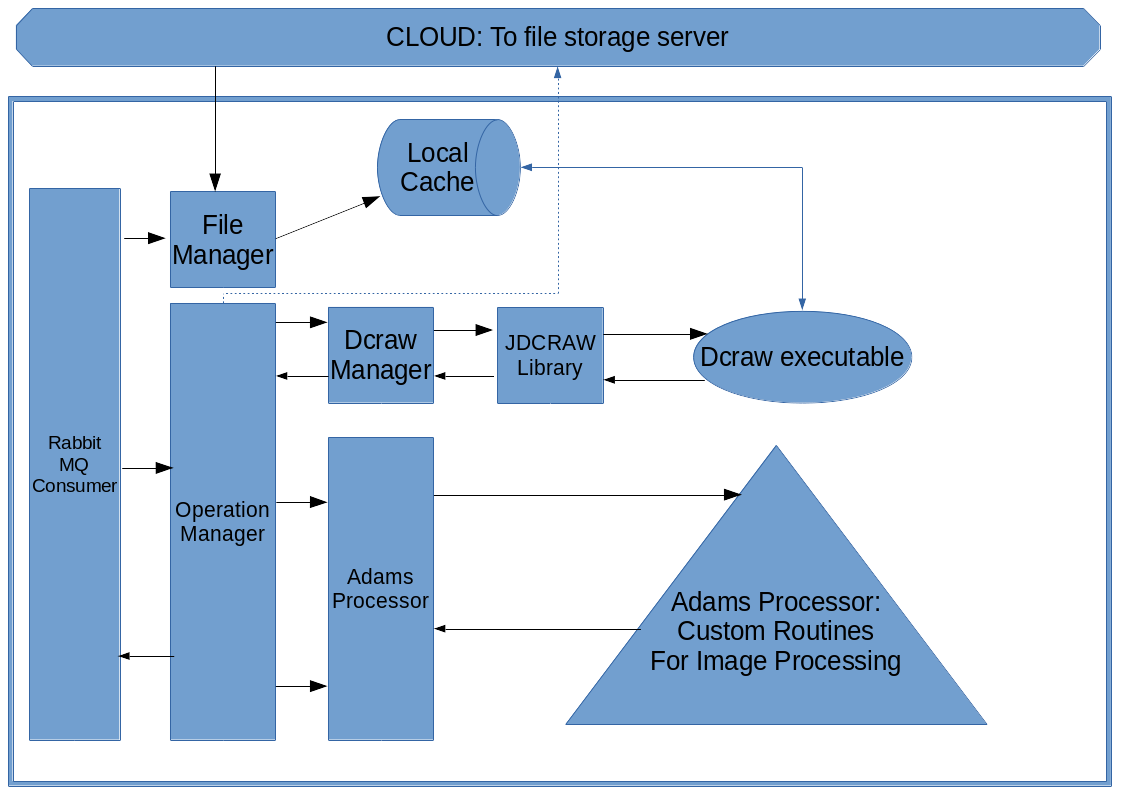
\includegraphics[width=\linewidth]{renderserverdiagram}
    \caption{The structure of the render server. The local cache is simply stored on the server local filesystem.
    RabbitMQ is a message queue - every single render job is added to the message queue, and the render servers take a job from the message queue
    to process. There are two queues, one to store jobs to process, others to store the results of jobs. When a job is finished, the result is added to the second
    queue, and this is then passed to the user.}
\end{figure}

\subsection{Adams Processor}\label{AdamsProcessor}
The Adams Processor, named after the famous photographer Ansel Adams (known for his black and white film landscape photographs), 
is the name given to the main routines powering our application. This deals with processing the image after generating the RAW image.
\subsubsection{Gamma Correction}
% Impmenetation
% formula
% lookup table
The process of gamma correction involves taking the RAW image, which by default has a linear tone curve (gamma of 1.0), and
mapping the colours to a different tone curve.

The function $f$ is used as a transformation from the image, to the gamma correction image. $f$ is defined as:

$$f(\gamma, v) = 255 \cdot \left( \frac{v}{255}\right)^{\gamma} $$

In the above definition, $v$ is the brightness value of one cell of the image, where $0 <= v <= 255$. First, we transform the
brightness of the individual channel (red, green or blue) to a floating point number, by dividing it by the maximum value for
the channel, which is $255$. Raising this to the power of the gamma factor applies the transform, and then multiplying it by $255$ converts the
target floating point representation back to the representation of a standard image (to be stored in a byte per channel).

On the implementation level, the best approach is to use a Lookup Table, with an input of the RAW image components (in our case, Red, Green and Blue),
and an output of the adjusted component values in accordance with the gamma correction function. The benefit of using a lookup table, rather than calculating
the gamma value for every single possible value, is that one doesn't need to calculate the same piece of data more than once (as bright regions, or dark regions might
potentially have the same input values). 

% \textbf{TODO: DIAGRAM SHOWING WORKFLOW OF THE LUT VS CALCUATING FUNCTION}
\subsubsection{Noise Reduction}
% Gaussian vs Mean
% Kernel Size
% Details
% Java Implementation Problems
Within an image, noise can be introduced by various means, including excessive ISO settings. Therefore are several different
types of noise, including Amplifier Noise, Salt-and-pepper noise, Shot noise, Quantization noise, on-isotropic noise, speckle noise
and periodic noise. 
\cite{NRandFiltering}


% Mean filter suited for random noise like Gaussian or Uniform noise. page 233
% Median Filter: less blurring, more detail. Good for bipolar and unipolar impulse noise. page 234

\paragraph{Amplifier Noise}
    This noise typically occurs with different sensitivities for different channels (e.g. red, green and blue detectors have
    different sensitivities). \cite{NRandFiltering}
    This can be removed by applying a Gaussian Blur. \cite{DigitalImageProcessingTextbook}

\paragraph{Salt-and-Pepper Noise}
    This noise is random noise, where random pixels might differ greatly from their neighbours. This noise can be caused
    by dead pixels on the camera sensor. \cite{NRandFiltering}
    
% \paragraph{Additive Noise}
% Spatial Filtering \cite[p.~231]{DigitalImageProcessingTextbook}



\subsubsection{Unsharp Image Adjustment}
    % Mean vs Gaussian
    % algorithm for doing this
    % implementation
    Unsharp Image Adjustment (masking), is one way of sharpening images.

    Given an input 2D image $I(x, y)$, applying a Gaussian Blur to this image will yield another image $I_{smoothed}(x, y)$.
    By doing a simple calculation, we can calculate the value of the mask $g(x, y)$. The parameters of Gaussian kernel size and 
    sigma can be used as additional parameters.

    $$g(x, y) = I(x, y) -  I_{smoothed}(x, y)$$

    By using this, one can then sharpen the image by using the output of this:

    $$I_{sharpened} = I(x, y) + \lambda \cdot g(x, y)$$.

    Here, $\lambda$ is defined as the amount in the Unsharp filter.
    
    \cite{Unsharp}

    When using the RGB colour space, with Unsharp on each individual channel, the colours can appear warped, so using the HSL colour space instead
    can reduce this, and also reduce the computation. The HSL Colour Space is a way of storing images, storing the Hue, Saturation, and Luminance
    for each pixel. The hue represents the colour, the saturation represents how prominant the colour is (the purity), and the luminance controls 
    the perceived lightness of the colour. This conversion is beneficial because only the luminance channel needs to be modified, rather than all three channels.
    However, one key problem is that the process can yield values of luminance (L) that exceed the $0 \le L \le 100$ range in the colour space.
    Furthermore, if this step isn't carried out, clipping can occur, which yields an overall loss of image data, something that isn't desired in a RAW editor.

    This problem can be solved by normalizing the image, by a process called contrast stretching. The max and minimum luminance values are found across the
    entire modified image, and these are used to scale the luminance values. Using standard Contrast Stretching does work, but at times tonal curves can look weird. By manually applying gamma though, this problem can be
    solved.

    One major problem regarding the Gaussian filter is that the user can potentially choose a large Kernel size, which results in increasingly lengthy
    periods to process. The alternative is to associate the SIGMA value of the Gaussian with the radius, detailing the standard deviation (spread) of the
    Gaussian over a fixed kernel. The Mean blur filter remains as before (though this feature is disabled through the web interface, as Gaussian is
    primarily used).

    One problem encounted in implementing this was lack of HSL support built into Java. Instead, an implementation of an HSLColour converter, was used,
    as documented in \cite{HSLImplementation}
\subsubsection{White Balance Adjustment}
    % Based on gains
    % control RGB components.
    % each one has multipliers
    Each colour image is made up of a variety of individual images, which are placed together
    to produce the colour images. These are the Red, Green and Blue masks.

    When one adjusts colours, our aim is to mix these three images together with a variety of different
    amounts, so that the overall image produced blends them together to create white (rather than an orange).
    The white balance control here can be adjusted further to tint the entire image.

    This is important in photography, as light sources don't always emit a uniform white light, but rather have some
    colour tint to it. As a result, the image that is captured will have colours appearing incorrectly (whites will appear 
    orange in some cases, or other shades). This effect can be removed in editing, but carrying out White Balance adjustment, also
    known as colour adjustment.

    In order to do this, we can simply scale the components of the internal camera RGB model, which can be done
    by adjusting the coefficients of these channels, which create a final colour image. In \cite{WhiteBalance}, \citeauthor{WhiteBalance}
    found that less distortion of colours was produced when using the camera RGB representation rather than monitor based
    RGB, as we are using the RAW format, we can store the camera representation, therefore producing less distorted colours
    as a result.


\subsection{Improving performance of fetching RAW files}\label{LocalImageCaching}
One of the biggest sources of delay in our system is the necessity to obtain RAW files. The user
provides a URL pointing to the RAW file in their render request, and then the system downloads the file
from that URL to use as the RAW file. Doing this for the same image constantly is very time consuming, and
as the user will likely be making many edits on the same RAW file, many downloads will be needed.

Therefore, implementing some form of caching is needed, to ensure that this download step only occurs once,
and then afterwards the cached RAW file will be used. Caching works in this situation, as when rendering,
the RAW file will not change at all (it's read only from our point of view), meaning that we obtain the
maximum quality through edits.

In order to do this, we need to save the image to the render server local disk, without any filename collisions
(where two different RAW URLs are cached to the same filename on disk).

The solution to this is to use a Universally Unique Identifier (UUID).
% Source https://docs.oracle.com/javase/7/docs/api/java/util/UUID.html

Our method uses the RAW file URL as the basis for the UUID generation, generating a Type 3 UUID based on the full path specified.
When downloading a file, the system first generates this UUID filename, and checks the local filesystem. If the file is present, then it
is already cached, and therefore the cached version is used. If the file isn't present, then it isn't cached, and a file is downloaded, and 
written to a filename based on the UUID (in this case, the format will be UUID followed by the extension). Type 3 UUID generation is based on
the MD5 hashing algorithm, by generating a 128 bit UUID. The hexadecimal representation (ignoring the dashes), is used as the replacement filename.

% For which type we used, reference the Java documentation
% TODO find reference for how Type 3 works

For a large number of RAW files being processed, using Type 5 UUIDs might be more suitable (as the algorithm used is SHA1 with a larger entropy), but
for a prototype use with few image URLs, this is more suitable.
% TODO find source for UUID probability of collision with MD5 Type 3 UUID vs Type 5. NEED SOURCE!!!

One other concern is the possibility of deleting files. While this is a grave concern typically, the current system doesn't have a time decay of caching,
simply because RAW files might be worked on over a period of days, and furthermore as the system is stateless, all files stored on the local system shall be
deleted regularly (configured inside Docker). Restarting render servers regularly is ideal, as this way we prevent memory leaks from the Java BufferedImage implementation
which have been minimized in our implementation but not completely eradicated.

\subsection{Web Editor Functionality}
% While render server does all the rendering, basic functionality of an editor should be present in the example
% cloud editor, for  testing.

% Implementing an Undo system: algorithms, data storage.
% User interface: sidebar with less cluttered nature.
The web editor itself provides an interface to the RAW Editing Service. Rather than
manually adjusting the settings and sending requests to the service, the parameters shall
be controllable through a Graphical User Interface, with the image result also being displayed
on the screen.

Furthermore, one must be able to undo and redo particular tasks. This is because the RAW editing
process typically requires refining parameter values, testing, and then opting to use the previously
set value. Having an undo/redo system would make this easier.

\subsubsection{Undo/Redo Functionality}
Due to our implementation, coupling that with the nature of our system, no current undo/redo queue library
seemed to be quite an ideal fit for our system. Therefore, it's necessary to build our own.

The system should, on modification of any parameters, store the change in some data structure,
so that it can be reverted.

This entire system relies on using a stack. When a change is made (one change shall be made at a time),
both the name of the parameter edited shall be stored, along with the old and new values. This shall be
stored together in an object, and pushed to the stack. To undo, one simply needs to pop the stack, and
set the specified parameter (given by the parameter name) value to the old value specified. 

In order to enable redo functionality, we create an empty stack, called the redo stack. When the undo function is called,
the object popped from the stack is also pushed to the redo stack. If the redo queue is not empty, and a normal change in parameter
has occurred, then the redo queue is emptied (one can no longer redo).

There are also a few edge cases. If someone presses the undo button when there are no actions to undo, then nothing can happen,
as there is nothing to undo. The same is true for the redo button.


\subsection{Storing User Images}
% While editing individual images is ok, editing a selection of
% images would be more functional, allowing us to select server uploaded
% images, edit them, and export them.
While one can edit individual images by simply supplying them to the editor, they need to be accessed somehow,
preferably through supplying some URL, where the RAW image can be downloaded, and then used to edit an image.
The system shall be built to be as customizable as possible, by downloading images from a supplied URL in the request,
and this RAW image is downloaded (or cached to the render server), wherever the file itself is hosted. This way, we can
either supply a system for uploading/storing images, or the user can choose to use an image store elsewhere such as Amazon
S3, OpenStack Swift, or other storage backend. Our system simply uses the Django file system, which stores the file in an
uploads folder on disk.



\subsection{Managing a big system}
% Docker/DockerCOmpose for managing a massive distributed system.
% Docker automatic restart on error 
As our system design calls for a large number of individual components, managing all of these together can be quite complex.

One option is to write a script that deals with the setup of each individual component: web server, web services, render dispatcher, render servers (however many we need),
and message queue. However, if a component of the system stops working, that'll bring down the system entirely, and writing a script won't necessarily allow us to deploy the system
across several different machines.

Our solution to this problem is to use Docker. Each component in the system shall be given its own individual container (essentially a virtual machine), where
it is sandboxed to ensure that systems don't interfere with one another, and each container is networked together. Rather than manually setting up the networking,
one can use Docker Compose to automatically deal with the links between different containers, to ensure that private links between containers are set up, but these links
can't be accessed from outside the system. This method is preferable, as then one cannot access the message queue/other sensitive components directly. That way, only by sending
the proper request, will the system respond with an output. 

With a microservice architecture, and some element of load balancing is recommended, along with some method of deploying services together so that dependencies
are met. These lessons learned from \cite{Docker}, were implemented by implementing our message queue backed render server, to load balance requests,
and to use Docker Compose as \citeauthor{Docker}'s work also did.

% \textbf{TODO: INSERT IMAGE OF ARCHITECTURE HERE}

\begin{figure}
\centering
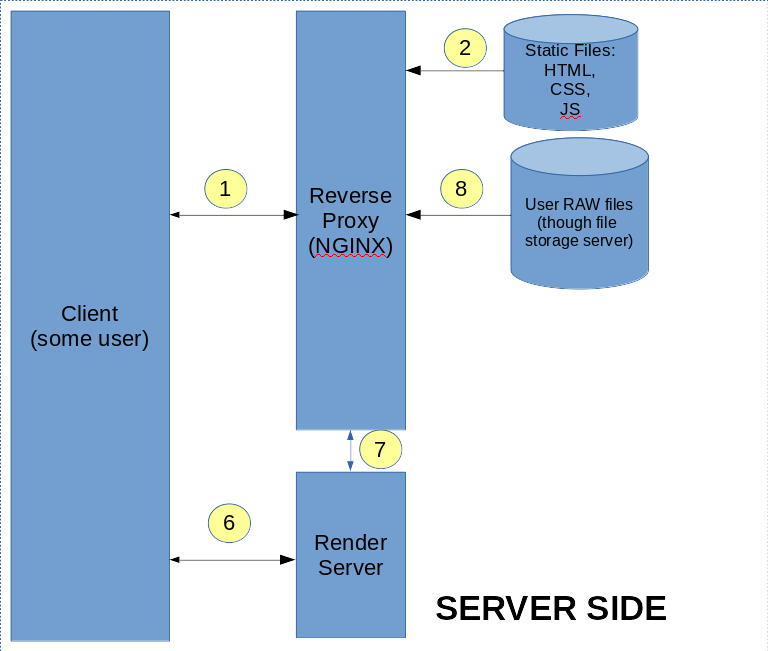
\includegraphics[width=200px]{architecture}
\caption{The architectural structure of the system. (1) File download of the client-side user interface. (2) Static files served through the web server.
(3, 4, 5) These were part of a system to allow users to upload and manage their collection of images. This was not implemented due to time constraints, and it was not directly related to the overall goal. (6) Socket.io communication
between the client and the render service, to generate previews and output images. (7) RAW Images are fetched from the web server.  (8) Test images can be served through the web server too.}
\end{figure}
% \textbf{TODO: DOCKER SOURCE }
\subsection{Unit Testing Issues with Image Processing}
% Can't just expect a given output, because each algorithm may change the image in a different way,
% and in some cases we are using floating point to do image adjustments. This causes some error, and therefore
% we won't necessarily get exactly the same image out.

For one to compare the output of the system with other RAW editors is not necessarily as easy as carrying out a bitwise-and  of the files, and finding the percentage
differences. While this might work if all systems use the same algorithms to do the same tasks, due to the proprietary nature of RAW image editing,
different implementations of demosaicing exist, yielding slightly different images, along with potential different ways of adopting equalization,
gamma correction and various other colour adjustments (for example, RGB gain was used to adjust the colours, while Lightroom instead uses chromacity).
It'll be difficult to use the same settings for every single system. Instead, a better solution would be to use a test image, and compare the adjustments
by eye between different applications, and use base cases or other expected behaviour to test the output of the system.

\subsubsection{Base cases include:}
\paragraph{Gamma Correction}
Setting $\gamma < 1.0$ will yield an image that appears whiter than expected. Setting $\gamma = 1$ should yield the input image.
Setting $\gamma > 1.0$ will yield an image that is darker in tone. 

% Using a gamma of zero will yield a completely white image. Using a gamma of 1 will yield the input image, for gamma correction.
\paragraph{Colour Balance}
Setting red gain to 1, and all others to zero will yield an image with only the red channel. Doing the same for green and blue should reveal the same.
This will ensure the algorithm is working correctly.

\paragraph{Exposure}
Exposure zero should yield a completely black image. Using a very high exposure should yield a completely, or nearly white image.

\section{Results}
This section outlines the results, to test the system against the deliverables and to compare it to other systems that are already in production.
The section aims to show that our solution works, and provides results to determine how well it works.
% this section presents the results of the solutions.  It should include information on experimental settings.  The results should demonstrate the claimed benefits/disadvantages of the proposed solutions.

% This section should be between 2 to 3 pages in length.
\subsection{Functionality Testing}
The functionality of the system can be tested by carrying out boundary checks. Certain parameters for different features should yield 
expected outcomes. For example, removing all blue and green channels should yield an image that's only red (with varying brightness in the red channel).

\subsubsection{Exposure Checks}
The boundary conditions here to check is with a zero exposure (yielding a black picture), a normal exposure (1.0), and a very high exposure.
The normal exposure should yield a normal image, while a very high exposure should yield a white image (or an image that's mostly white, with a few
bright spots). When testing, zero yielded an inverted colour, but with a small value near zero yielded the appropriate result.

% \textbf{TODO test exposure}

\begin{figure}\label{exposuretest}
    \centering
    \subfigure
    {
        
\includegraphics[width=75px]{brightnesspoint0001}
    }
    \subfigure
    {
        \includegraphics[width=75px]{brightnessnormal}
    }
    \subfigure
    {
        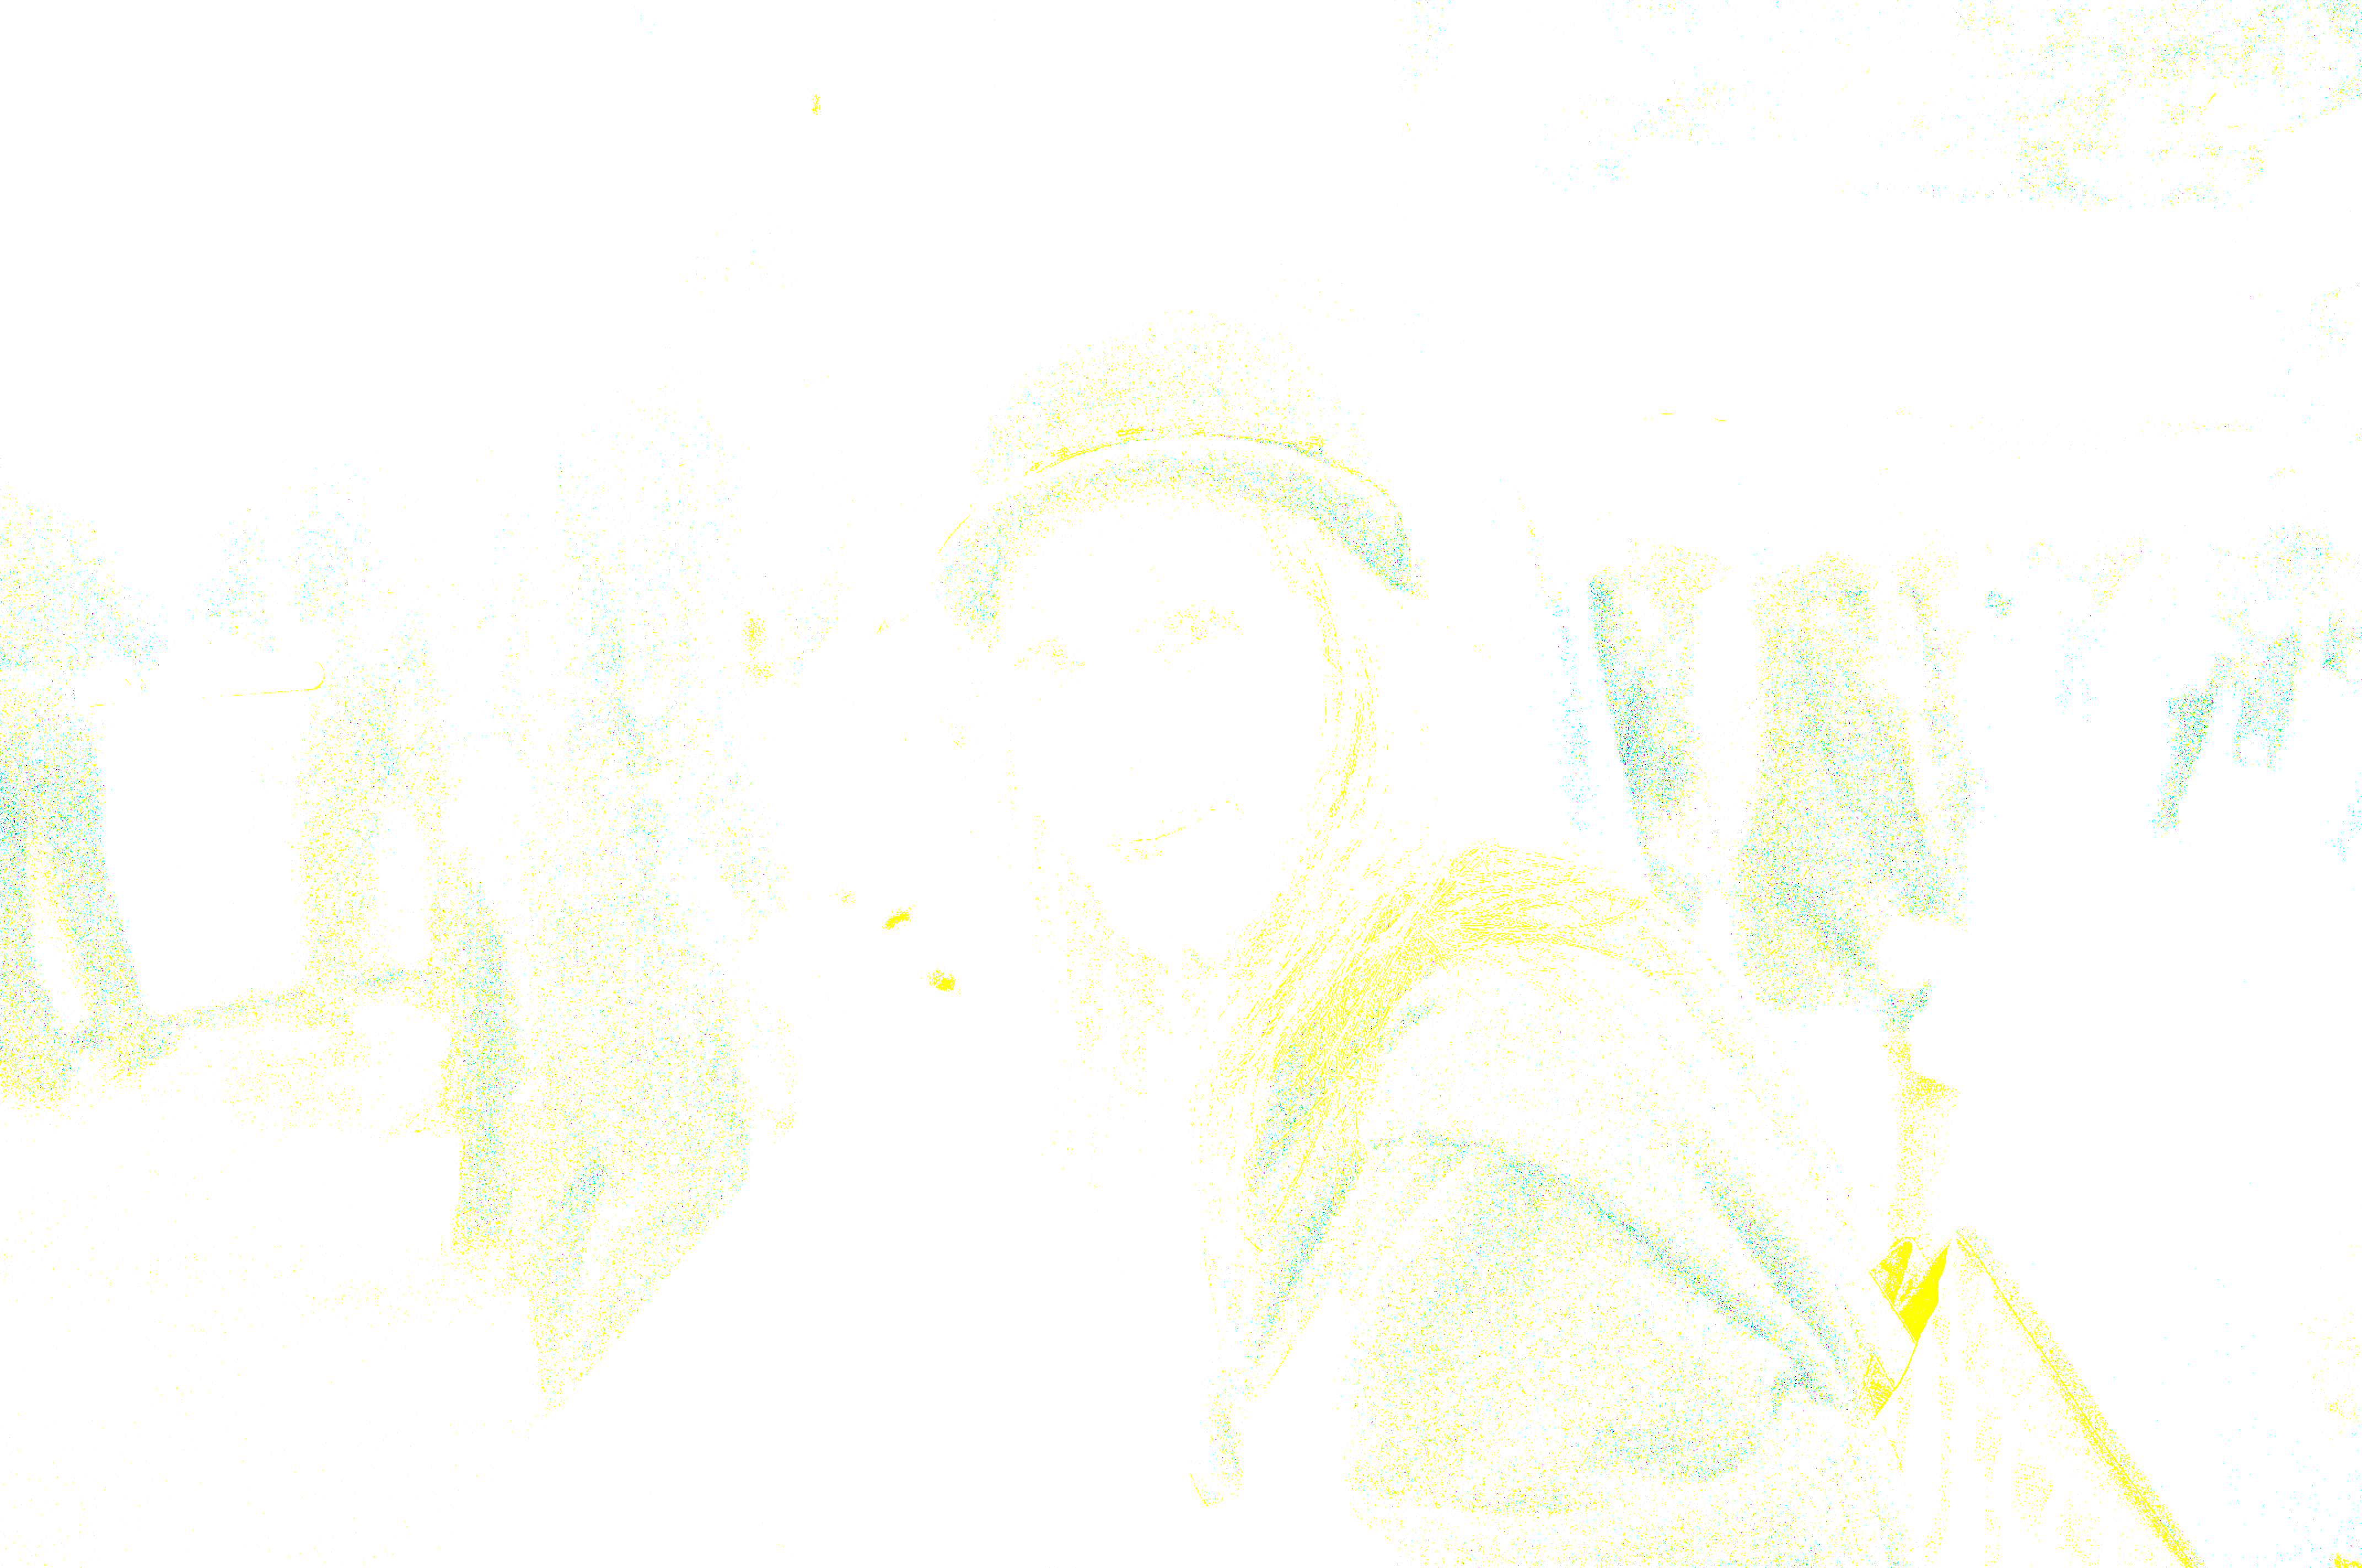
\includegraphics[width=75px]{brightness5000}
    }
    \caption{
        Test of Exposure Adjustment 
        (a) Exposure Level Small: 0.0001
        (b) Exposure normal: 1.0
        (c) Exposure level high: 5000
    }
 \end{figure}

\subsubsection{Colour Balance Checks}
Colour balance is controlled with red, green and blue gains. If we set only one of these gains to 1.0, and the other two to zero, we should
have a version of the image, but only with the specified colour, present: rather like a grayscale image but in one specific colour rather than black to white.
The results of this check can be found in Figure \ref{colourbalancetest}. These results show that the colour balance algorithms are working correctly.
\begin{figure}\label{colourbalancetest}
    \centering
    \subfigure
    {
        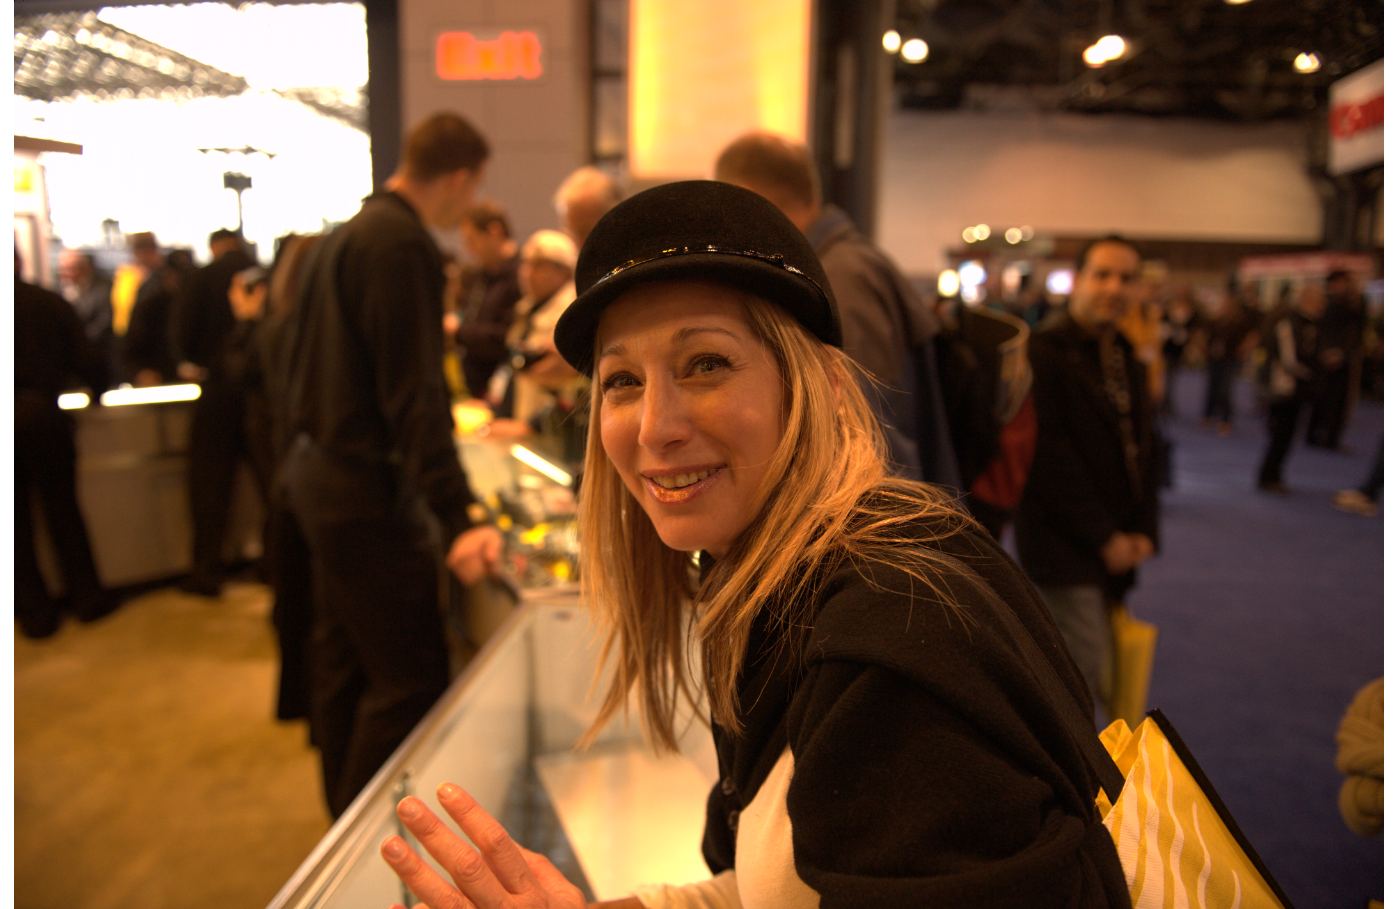
\includegraphics[width=75px]{colourtest_no_adjustment}
    }
    \subfigure
    {
        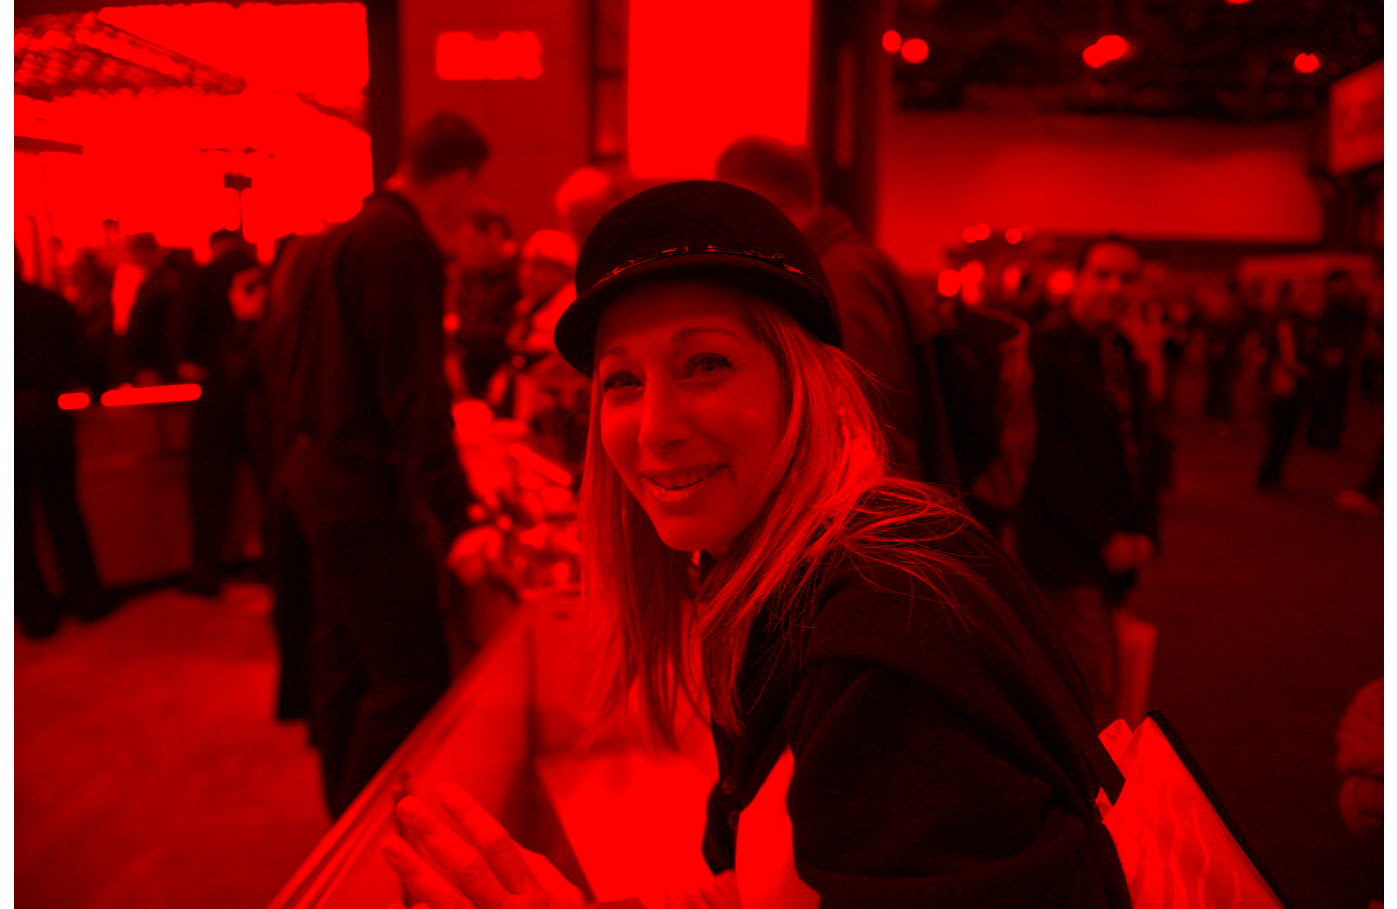
\includegraphics[width=75px]{colourtest_redonly}
    }
    \subfigure
    {
        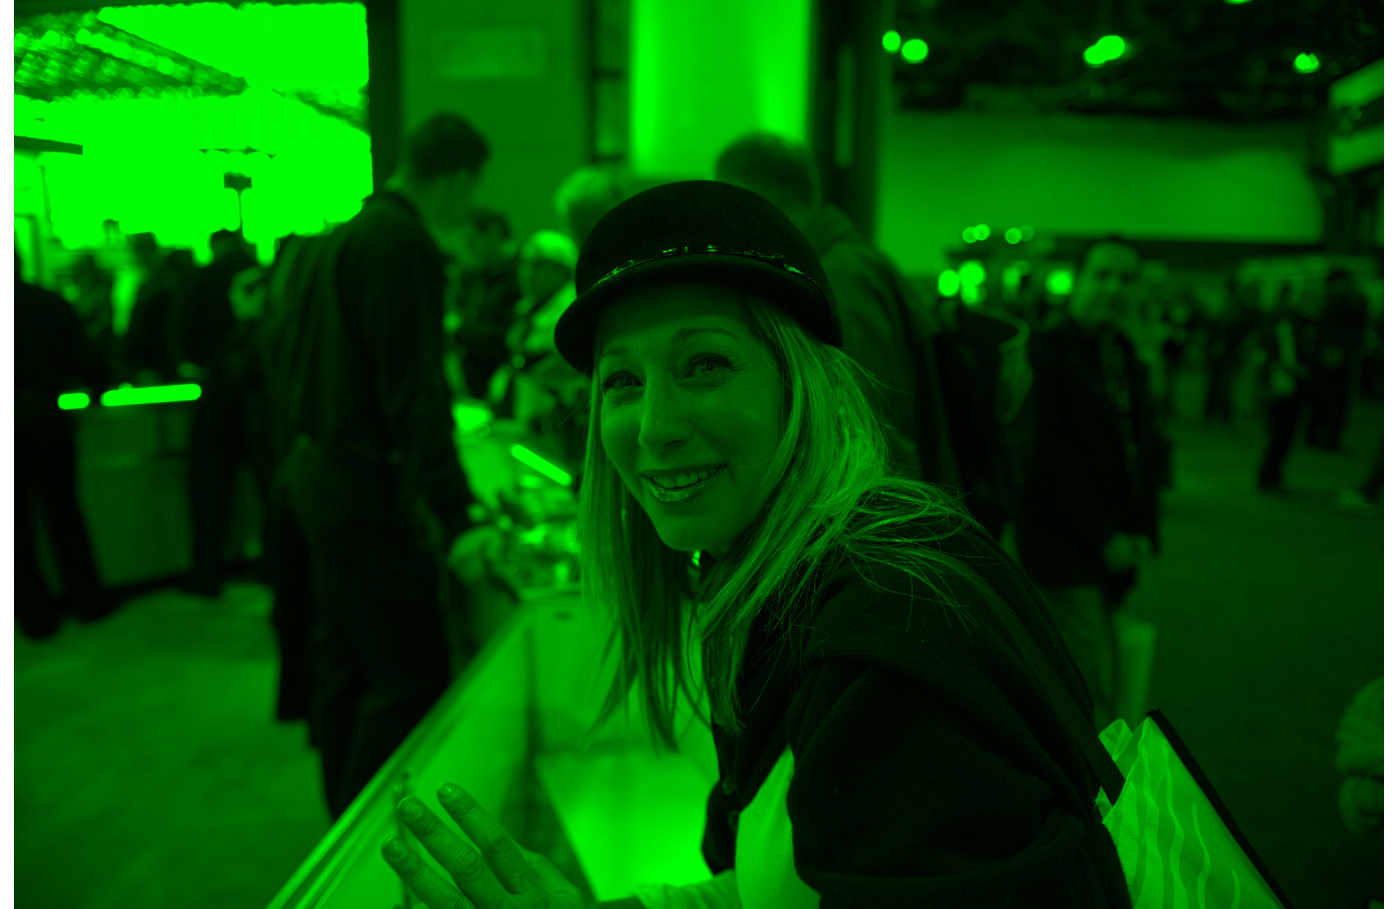
\includegraphics[width=75px]{colourtest_greenonly}
    }
    \subfigure
    {
        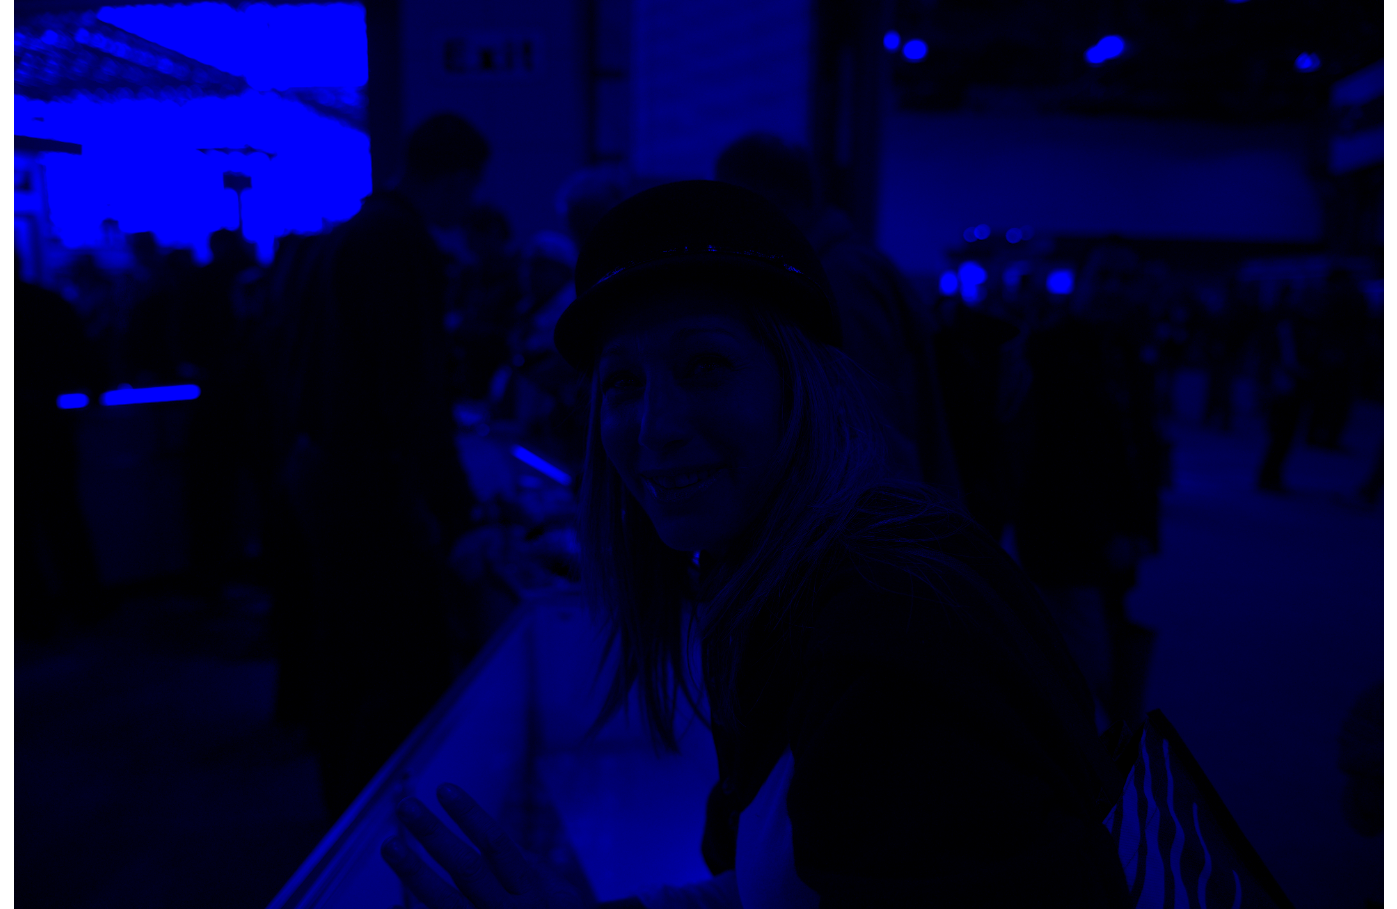
\includegraphics[width=75px]{blueonly}
    }
    \caption{
        Test of Colour Balance 
        (a) No Adjustment
        (b) Red only (green and blue zero)
        (c) Green only (red and blue zero)
        (d) Blue only (red and green zero)
    }
 \end{figure}

\subsubsection{Unsharp}
Enter a fairly high Unsharp radius (the sigma of the Gaussian), and amount. This should then yield an image with enchanced edges in comparison to the normal image without unsharp masking. As a reference
point, a specific part of the image should be used to compare the sharpness, to determine the
functionality of the implementation.

Reducing the unsharp amount to zero should cause the output image to be the same as the input image.


% \textbf{TODO test Unsharp}
\subsubsection{Gamma Correction}
Enter various gamma values in the range $0 < \gamma \leq 2$, and compare them. This should yield a noticeable difference in tone. With a gamma less than 1,
the tone will have more white colours, while with a gamma greater than 1, the one difference will be darker (with more darker colours than white). The
outcome of this test can be seen in Figure \ref{gammatest}. The implementation yields this expected outcome.

\begin{figure}\label{gammatest}
   \centering
   \subfigure
   {
       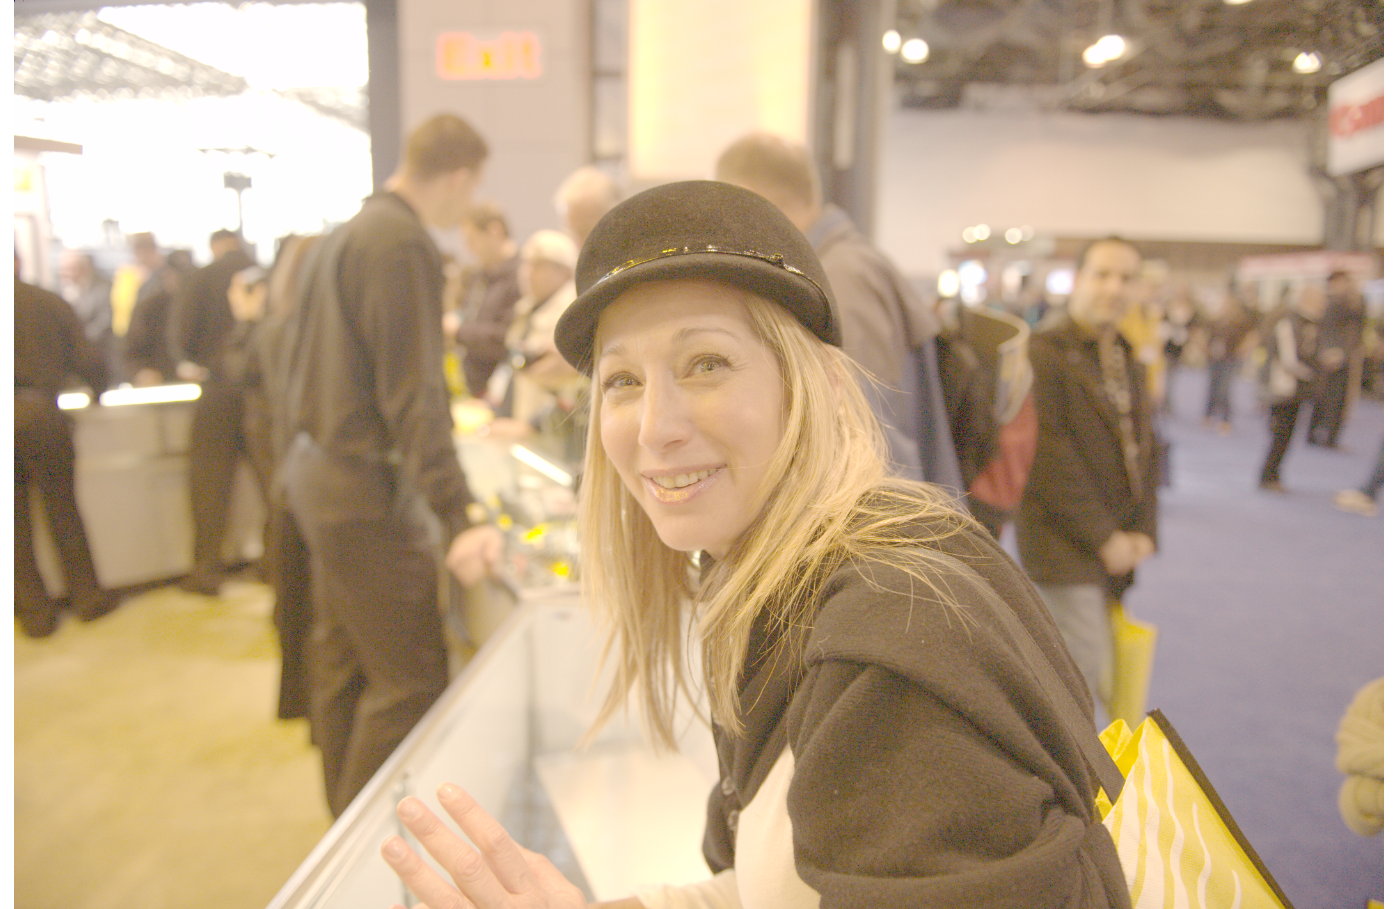
\includegraphics[width=100px]{gammacorrectionlow}
   }
   \subfigure
   {
       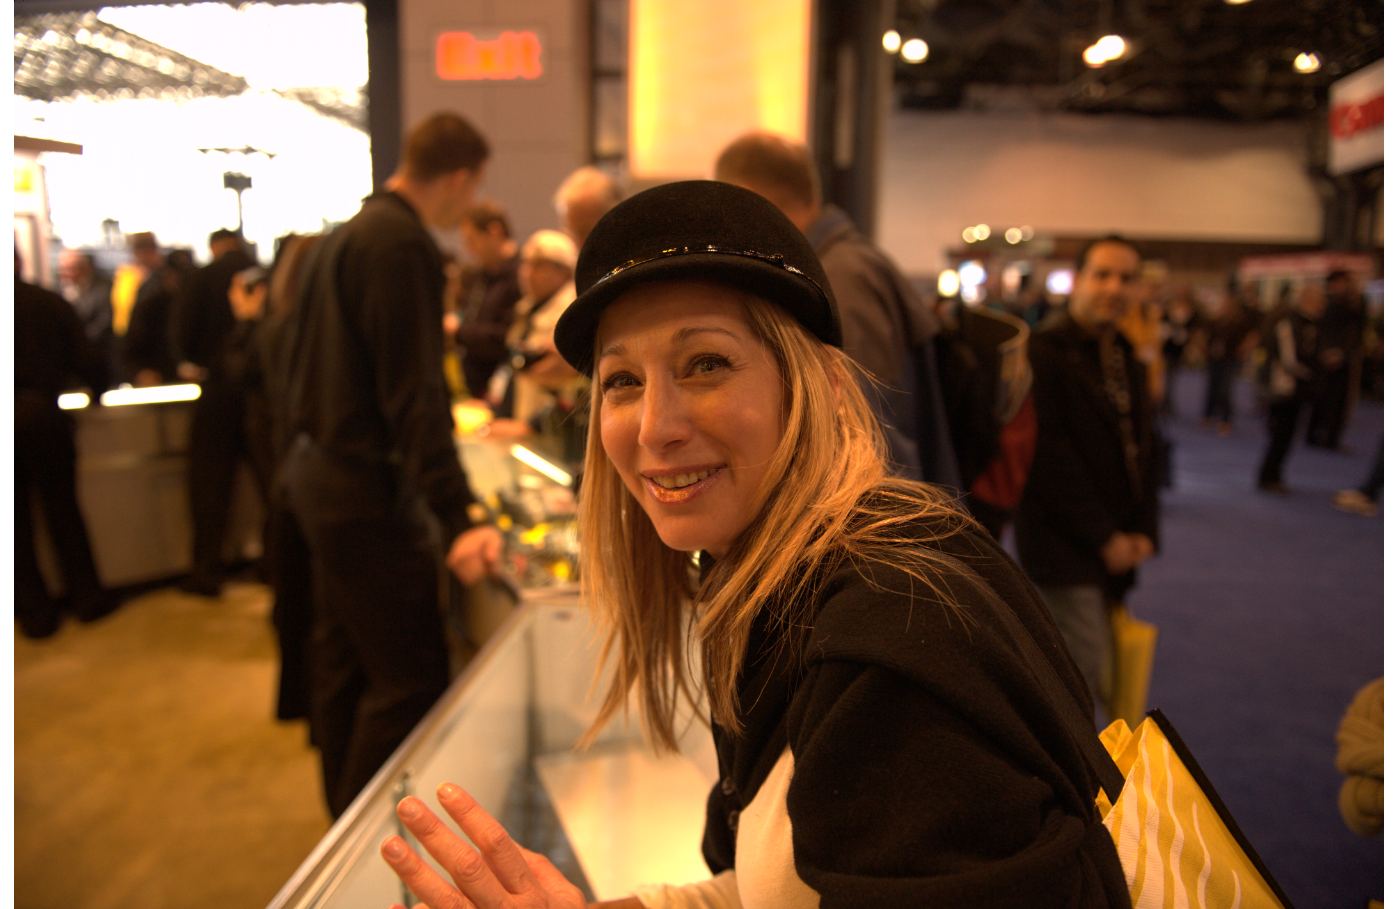
\includegraphics[width=100px]{gammacorrection_normal}
   }
   \subfigure
   {
       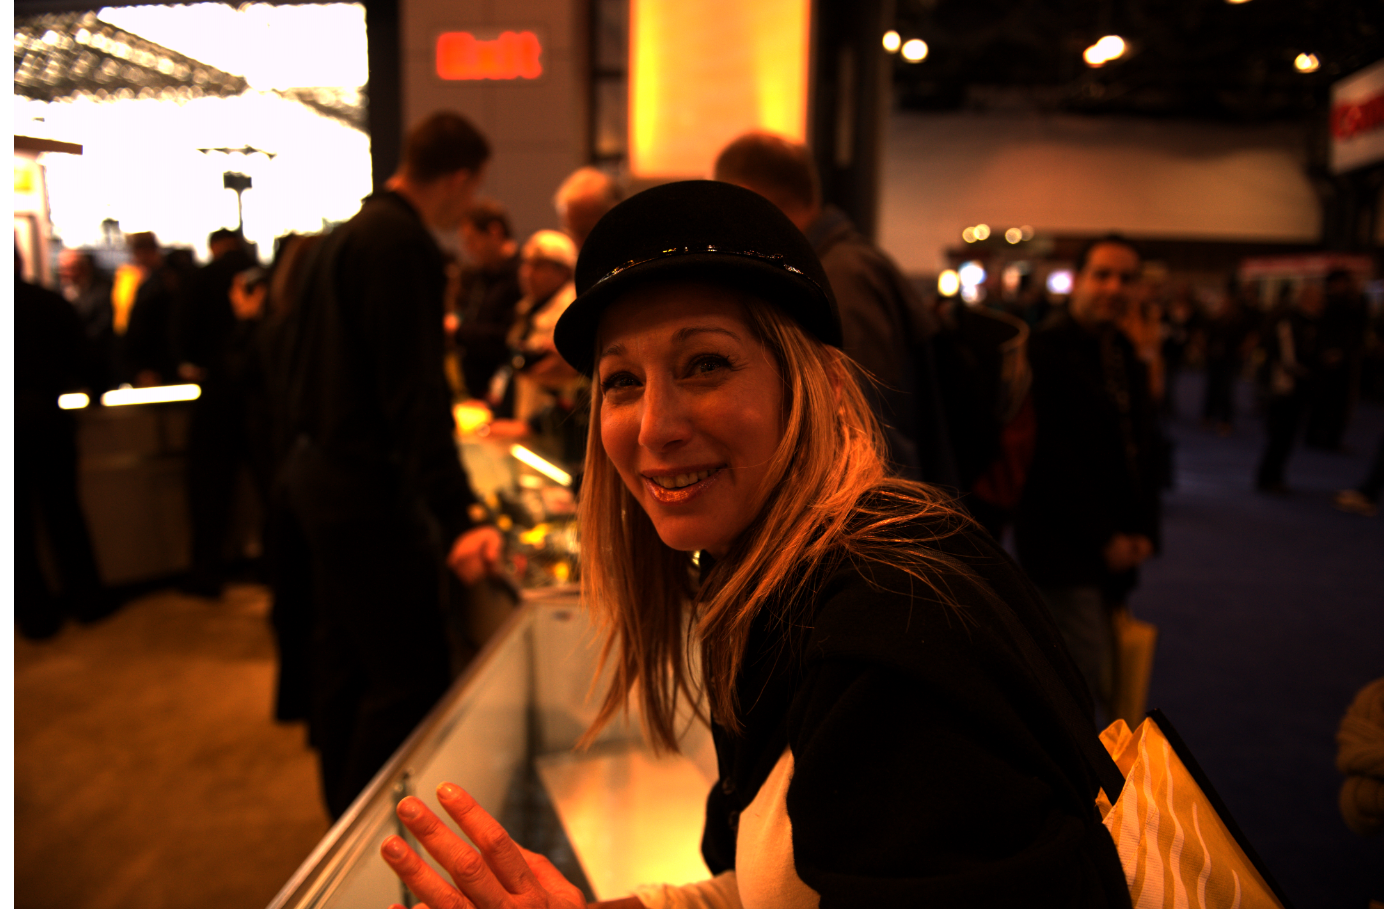
\includegraphics[width=100px]{gammacorrectionhigh}
   }
   \caption{
       Test of Gamma Correction output. 
       (a) $\gamma = 0.3$
       (b) $\gamma = 1.0$
       (c) $\gamma = 1.7$
   }
\end{figure}
% \subsubsection{Gaussian Blur}
% Test this by setting a high sigma value, with kernel size of 3. The expected outcome is an image that appears noticeably blurred.
% % \textbf{TEST Gaussian Blur}
% \subsubsection{Mean Blur}

\subsubsection{Histogram Equalization}
While the exposure is set, the exposure can also be automatically adjusted using Histogram Equalization. As this happens after the exposure (and all other processing)
we can test this by setting a fairly low exposure (not 0, but probably in the range of 0.5), and then applying Histogram Equalization. The expected outcome is a brightness
that's comparable to the image with normal (1) exposure.

% \textbf{TEST HISTOGRAM EQ}

\subsection{Comparison With Other Editors}
In order to evaluate the performance of the system, both in the output image, along with the overall system performance,
responsiveness (measured in delay in rendering an image), a set of different image manipulations were carried out on various
different RAW editors and our system. These were all run on exactly the same hardware, with the same Operating System.

The system specification can be seen in Figure \ref{SystemSpecs}.

\begin{figure}\label{SystemSpecs}
    \centering
    \begin{tabular}{| c | c |}
        \hline
        Processor & Intel i7-7700k, 4.2GHz\\
        RAM & 16GB at 3000\\
        HDD & 1TB Seagate Barracuda, spinning at 7200RPM\\
        Operating System & Microsoft Windows 10 with Ubuntu subsystem\\
        \hline
    \end{tabular}
    \caption{The specification of the test system.}
\end{figure}

Adobe Lightroom, RawTherapee, and Darktable were used to compare the performance of our system. For the comparison results,
a RAW sample was obtained from the D700 camera.
% \textbf{TODO reference RAW Samples Website}

\subsubsection{Test 1: Exposure Adjustment}
In order to compare exposure, various different exposures were used. Some by decreasing the exposure level, others by
increasing the exposure level, and leaving the exposure level at 1.0

% % \textbf{TODO test exposure}
% \subsubsection{Test 2: Gamma Correction}
% While the initial plan was to compare different gamma values, both Lightroom and RawTherapee do not allow for gamma factors to be
% manually entered, but instead require them to be controlled via a light adjustment on the user interface. As such, there isn't really
% a way of comparing the gamma correction output between the several systems

\subsubsection{Test 2: Sharpening}
While these are defined by different terms between software programs, we can still test the overall outcome.
Rather than deciding the quality of sharpening by how pronounced the edge is, it's instead done by comparing a portion
of the image (the brim of the hat), sharpened between different applications. The results can be seen in Figure \ref{unsharpcomparison}.

\begin{figure}\label{unsharpcomparison}
    \centering
    \subfigure
    {
        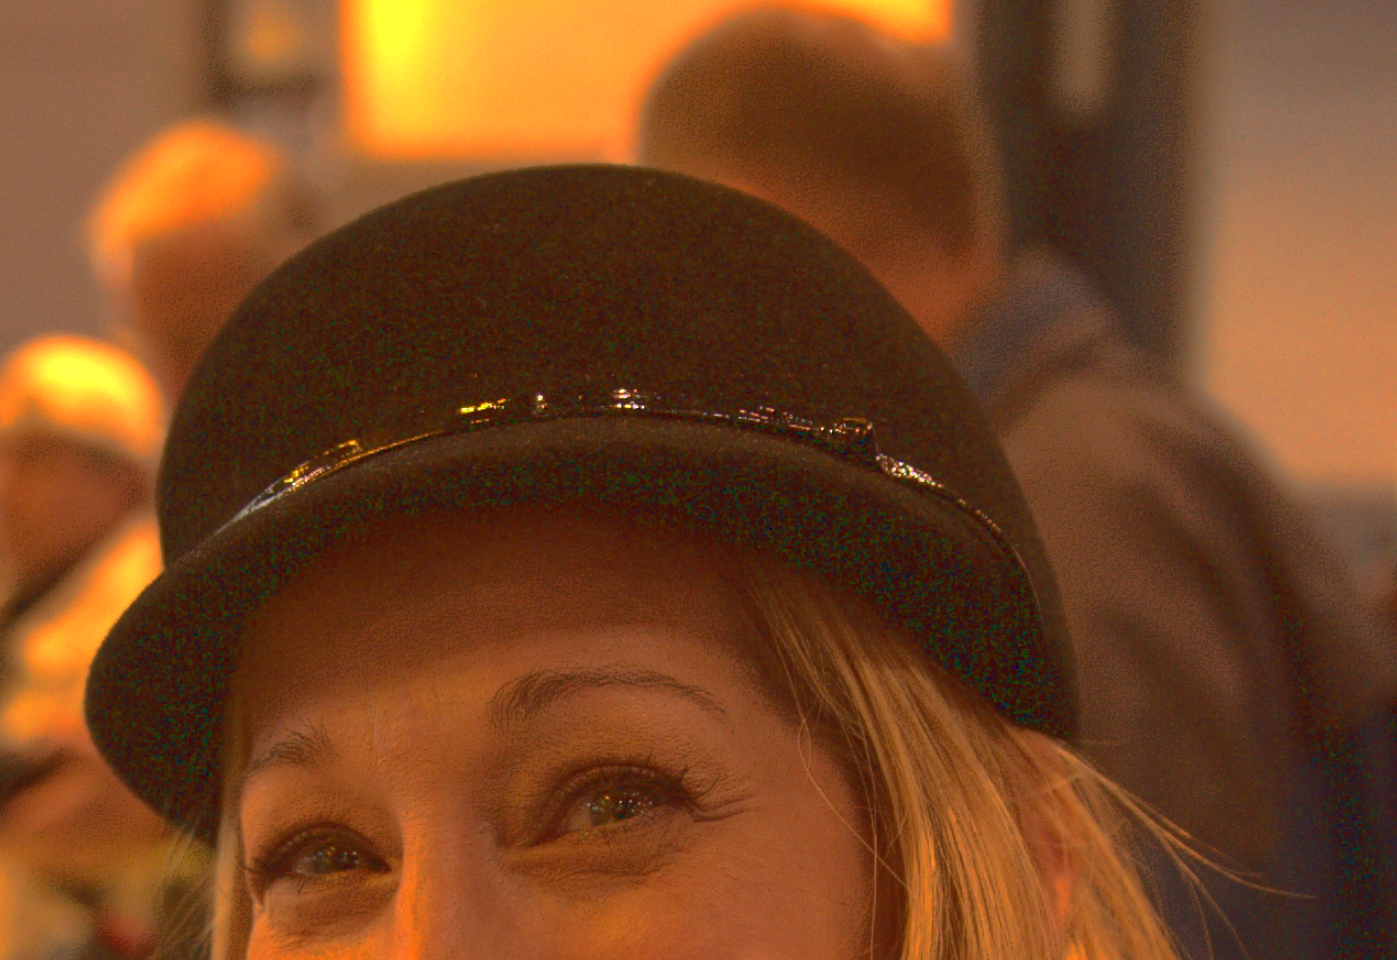
\includegraphics[width=100px]{rawflash_hat_sharp}
    }
    \subfigure
    {
        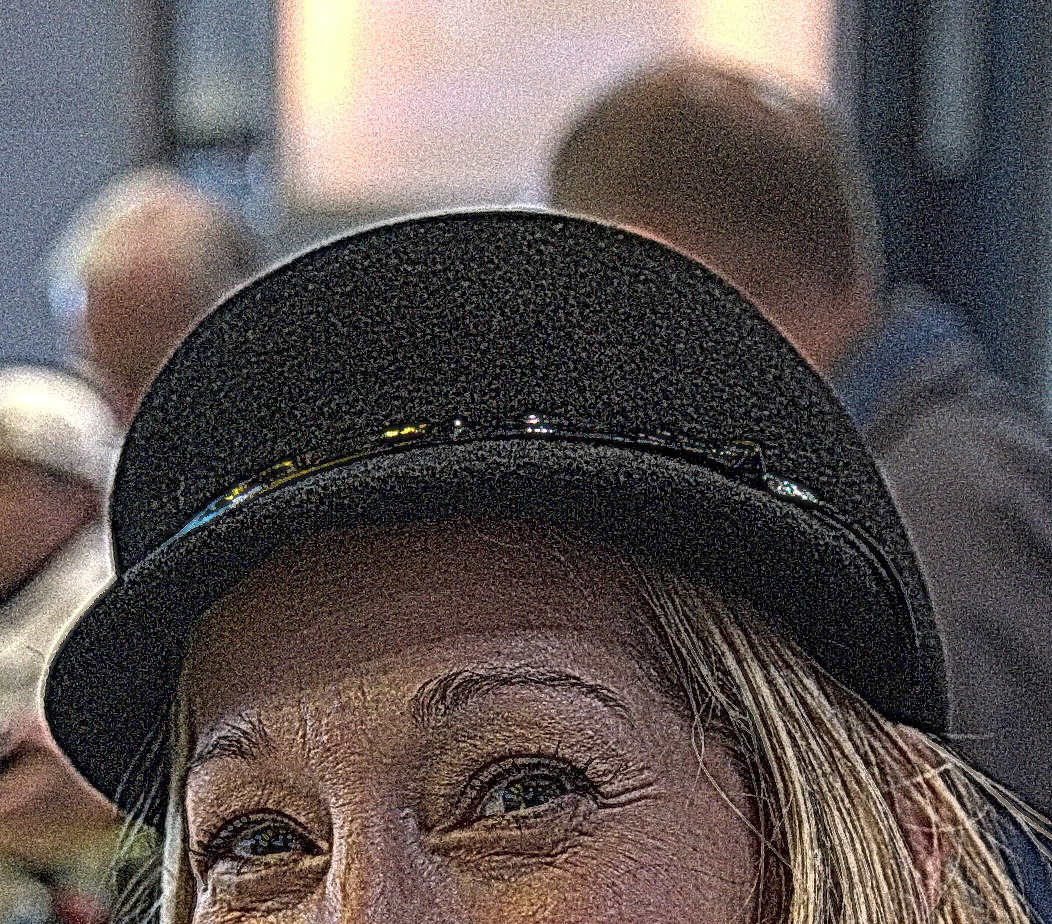
\includegraphics[width=100px]{rawtherapee_unsharp_max}
    }
    \subfigure
    {
        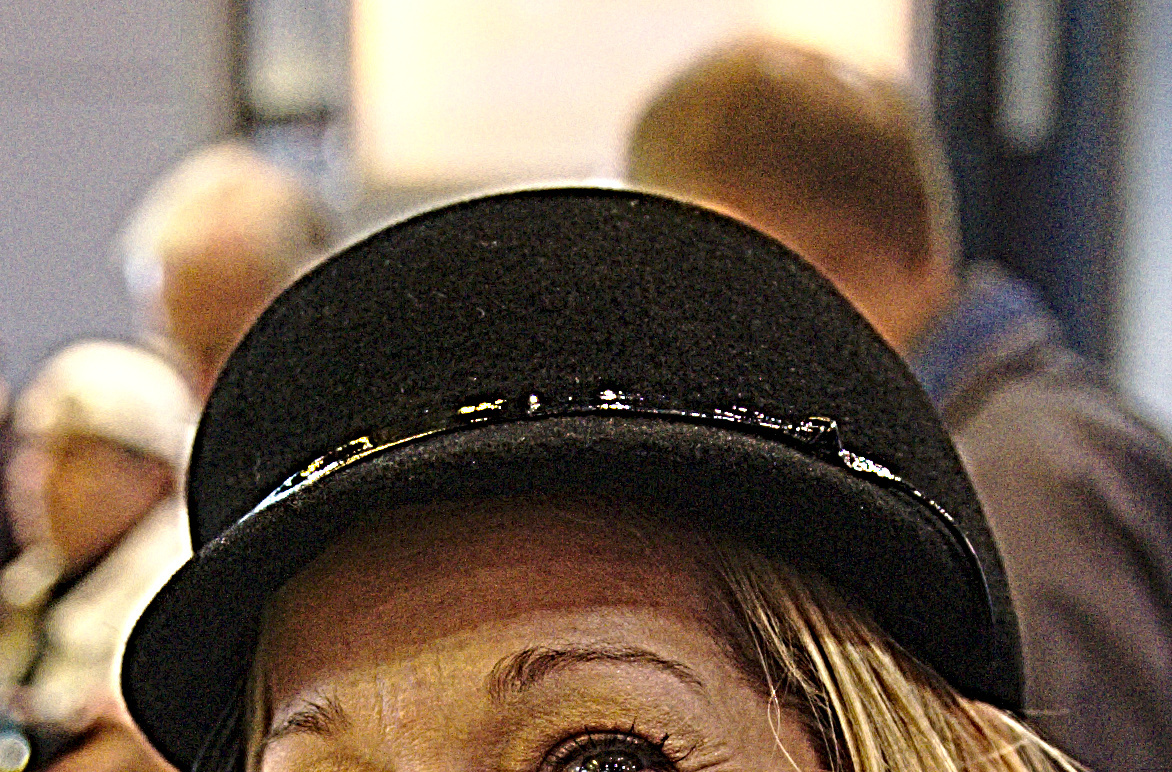
\includegraphics[width=100px]{darktable_unsharp}
    }
    \caption{
        Test of unsharp sharpening. The brim of the hat is used as the edge to compare. 
        (a) RAWFlash, our system
        (b) RawTherapee
        (c) DarkTable
    }
 \end{figure}


In terms of quality, while the other two systems do perform slightly better, our system does fairly decent job of sharpening
the image and enhancing most of the common images. There are a few colour differences between the systems, mostly due to internal
colour processing, but overall each one of the systems enhance the brim of the hat, making the line sharper and appear less blurry. 
Our system enhanced the edge enough so that it could be seen, but not so much as to make it too pronounced.

\subsubsection{Test 3: Colour Adjustment}
Colour adjustment is done by using the colour channels, and adjusting the different levels of red, green and blue that exist within the image.
Between all three systems that are being tested, the parameters that need to be set remain fairly constant (some use percentages, while others use decimals,
but they all represent the same transform).

% \textbf{TODO insert image comparison here}
\begin{figure}\label{colouradjustmentcomparison}
    \centering
    \subfigure
    {
        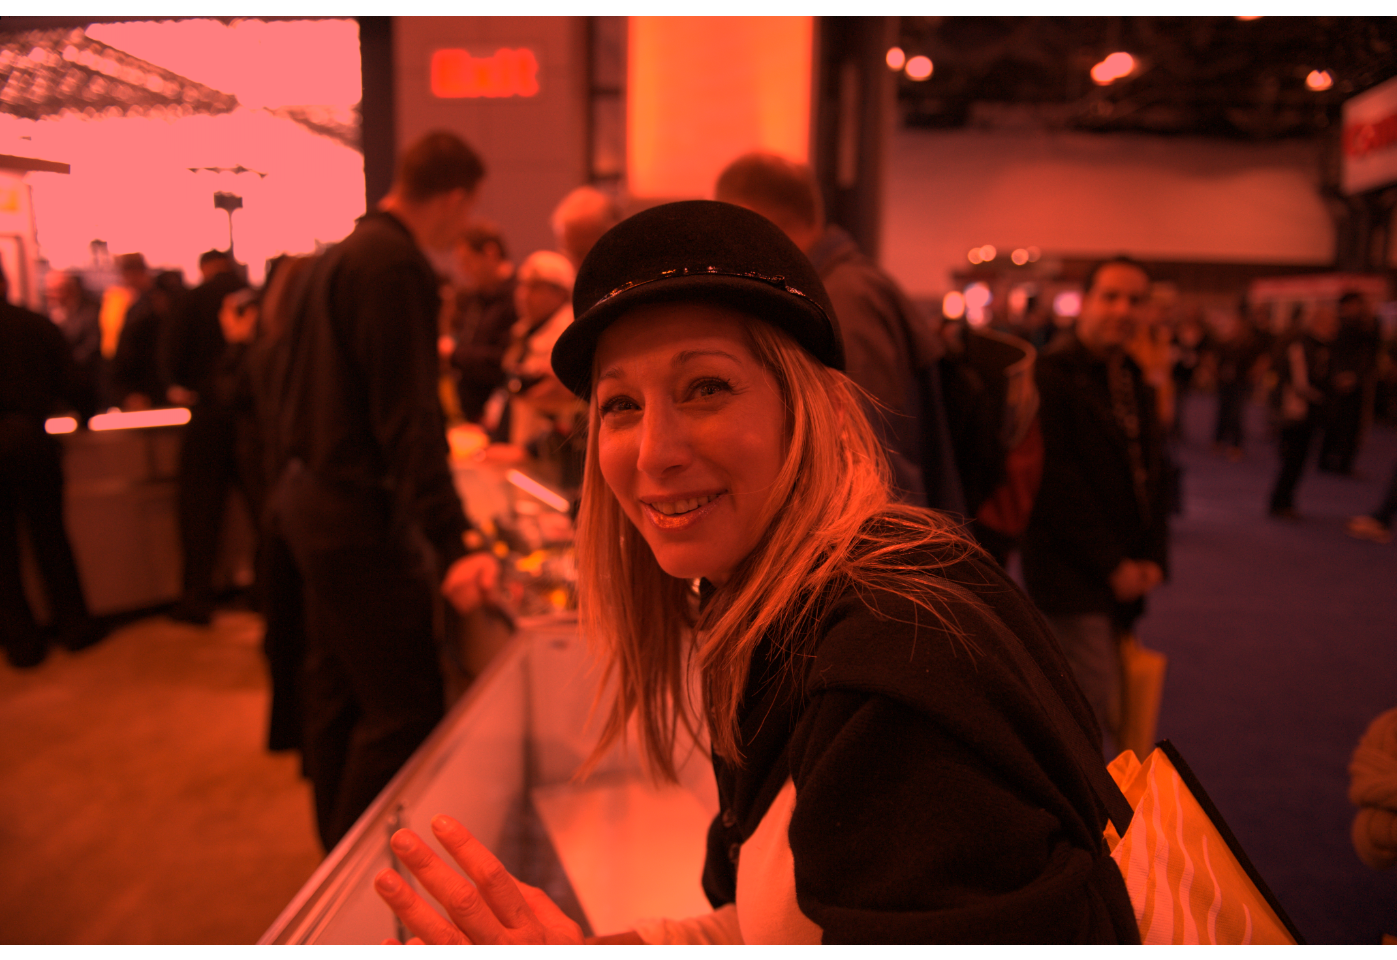
\includegraphics[width=100px]{rawflash_colour_adjustment}
    }
    \subfigure
    {
        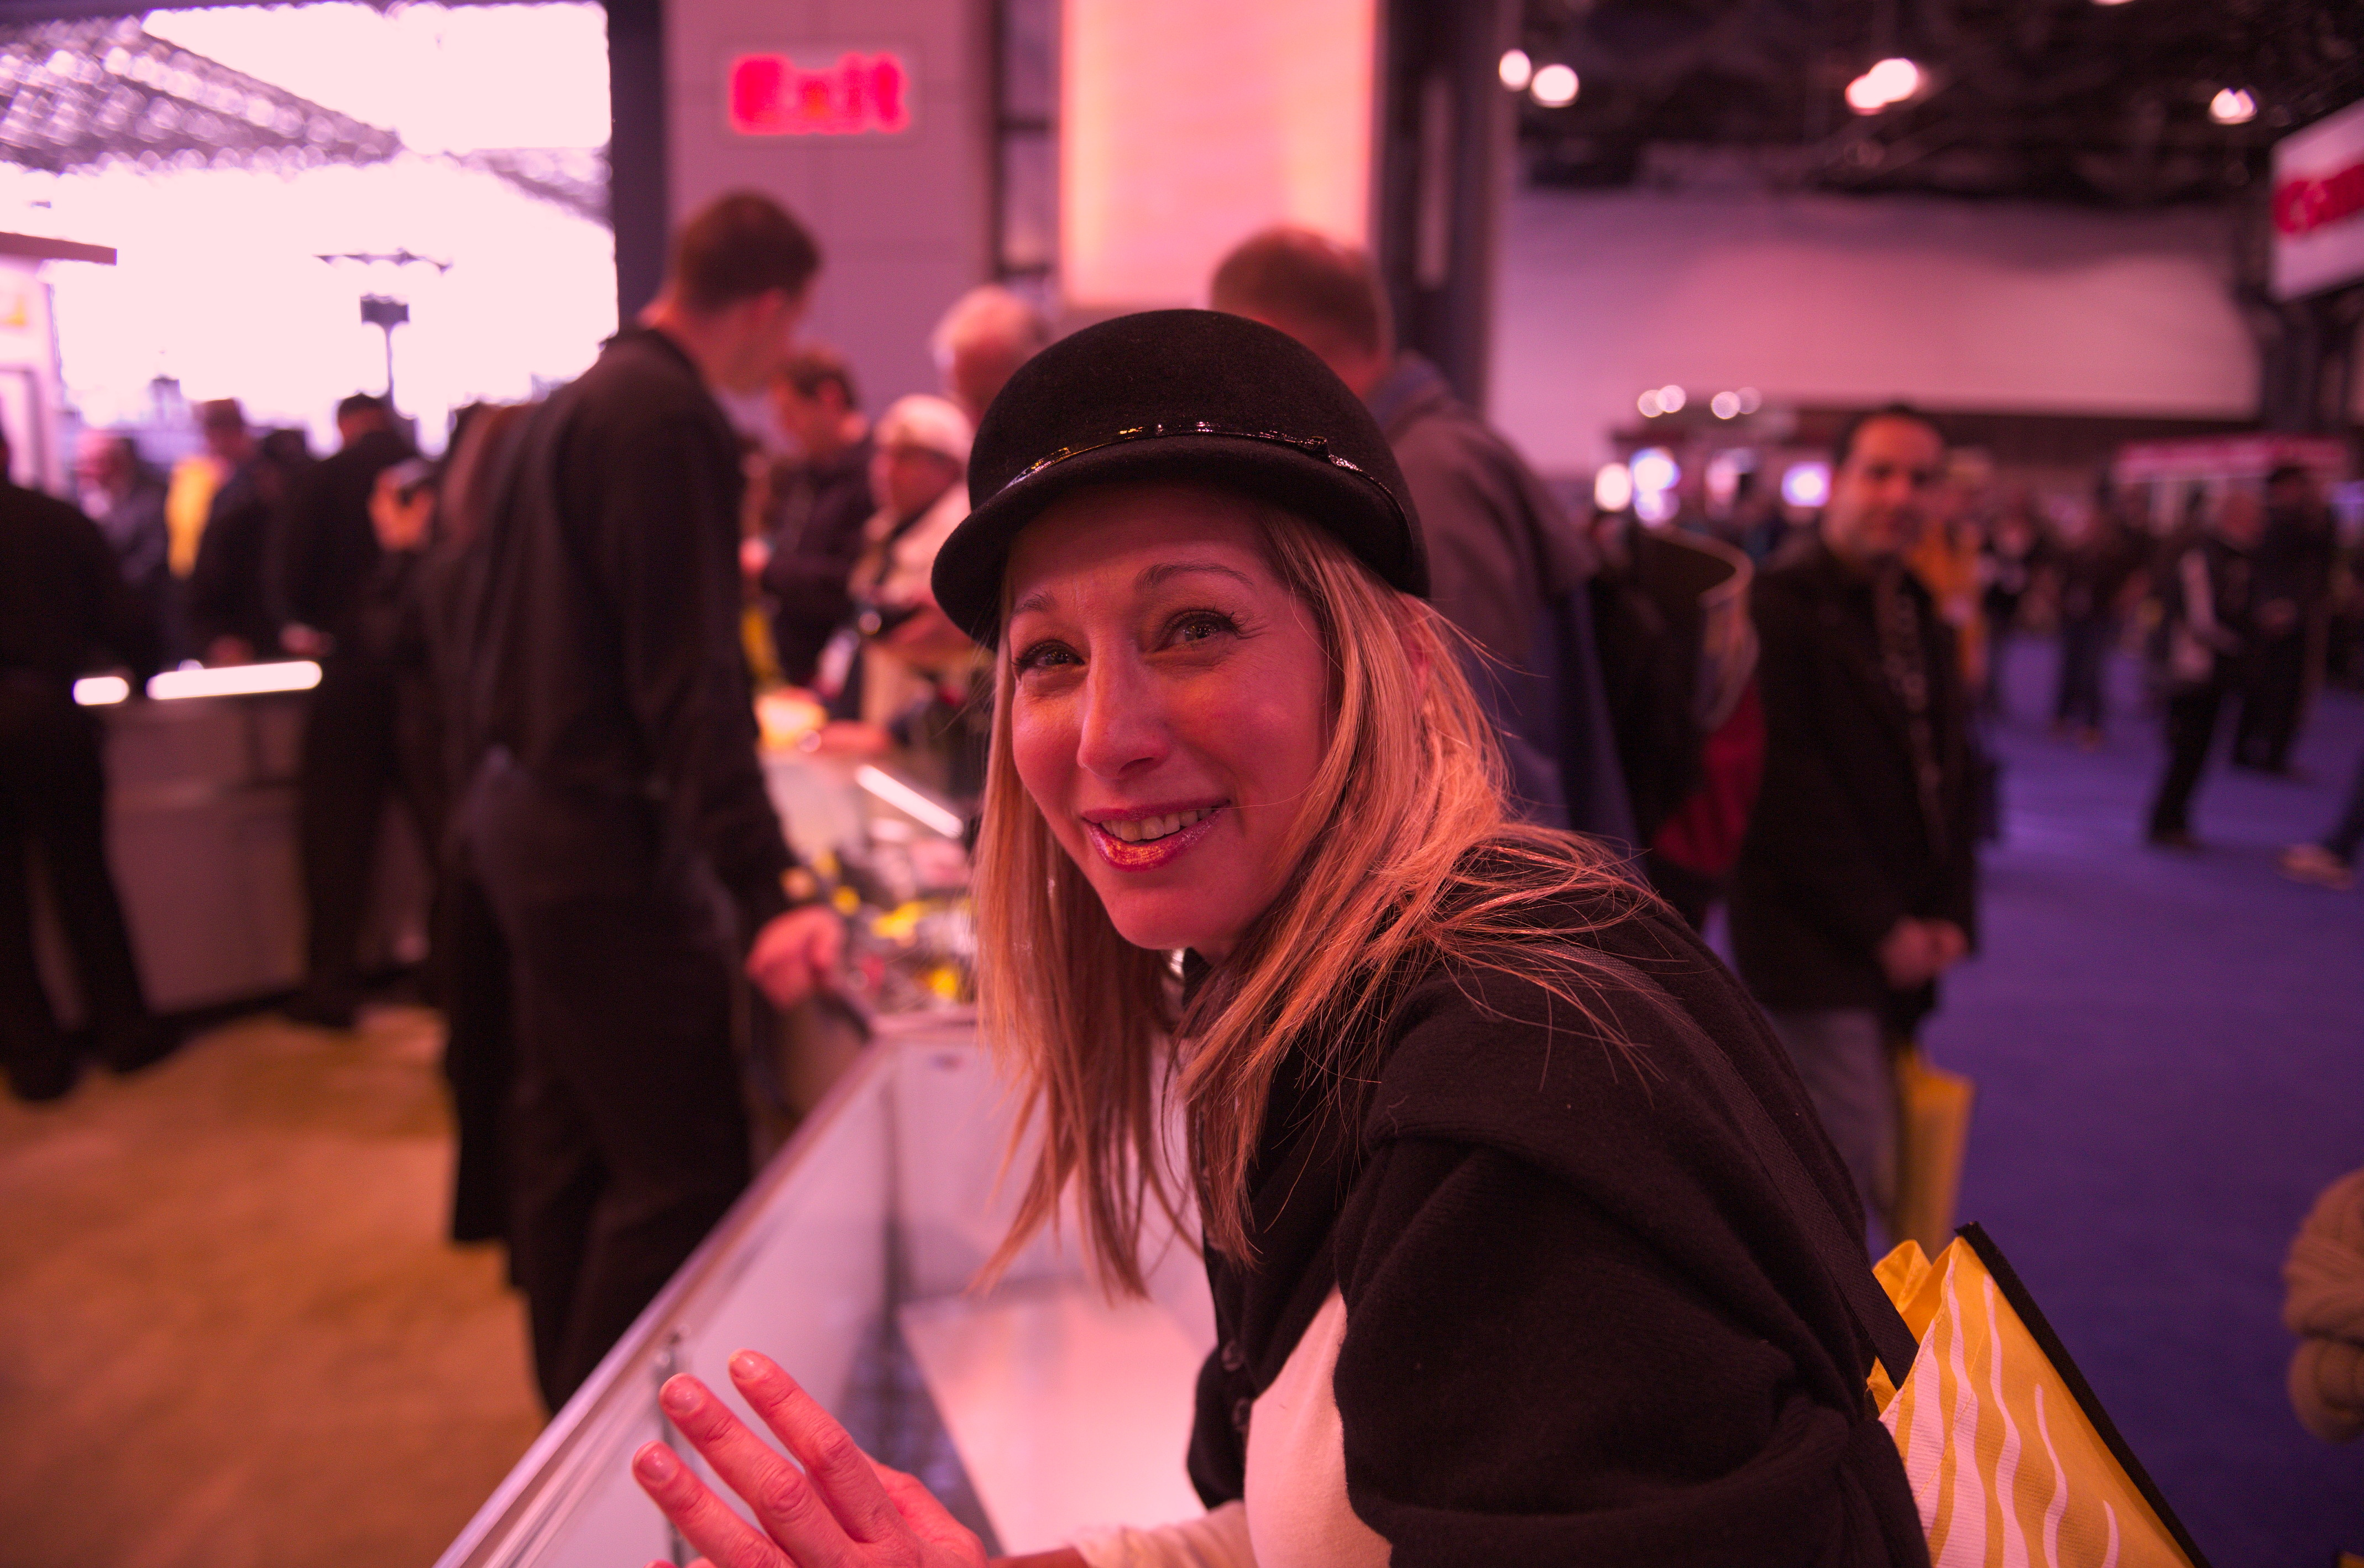
\includegraphics[width=100px]{rawtherapee_colour_adjustment}
    }
    \subfigure
    {
        \includegraphics[width=100px]{darktable_colour_adjustment}
    }
    \caption{
        Test of Gamma Correction output. 
        (a) RAWFlash, our system
        (b) RawTherapee
        (c) DarkTable
    }
 \end{figure}
In comparison to the other systems, they all perform in the same way. There is some slight difference in colour between them, as different colourspaces
are being used in different applications, and as such, colours are sometimes represented slightly differently. Compared to the original image however, our
system is certainly functioning.

\subsubsection{Test 4: Render Time}
One crucial test is to compare the time it takes to render an image. For the portable image editing workflow, this is key as editing typically involves
refining settings constantly throughout the editing process. For the use as a standalone image editor, this time should be fairly low, but for a RAW
image rendering service, this can be higher, as often RAW images can be edited in batch. The results can be seen in Table \ref{RenderTimeTable}.

\begin{table}
    \centering
    \begin{tabular}{| c | c |}
        \hline
        Application & Time Taken To Render (seconds)\\
        \hline
        RawTherapee & 0.3\\
        DarkTable & 0.3 \\
        RAWFlash & 7.3 \\
        \hline
    \end{tabular}
    \caption{The time taken between triggering a render and the image displaying on the screen measured in seconds.}
    \label{RenderTimeTable}
\end{table}

\section{Evaluation}
This section evaluates how well our system works, how well it solves the problem of RAW image processing as a service,
and how it can be applied.
% This section should between 1 to 2 pages in length.

\subsection{Application as a RAW Image Editor}
The system works well at producing images, taking the RAW images and adjusting exposure, colour, and adding sharpening, and exporting the final image.
The overall images produced are as expected, and the processing that is carried out on them is what is expected from the algorithms implemented.


\subsection{Application to Web Content Management Systems}
% Process of editing and uploading images
% RAW -> JPEG -> Upload -> Further compression/adjustments in CMS for web -> Output
% better to skip intermediate steps, meaning less computational effort on one end, less cost for
% expensive software.
When applying our system to web content management systems, or for other applications that require a headless method
of rendering RAW images, it functions well. With the CMS workflow, of uploading a set of RAW images, and having the system
process them in batch our system would work better, as this batch processing will often be done in the background, producing
the output that can then be stored, ready for use.

\subsection{Performance Issues and Improvements}
% Improvement by use of multithreading for image processing
% Java's build in Image Manipulation has a number of undocumented bugs.
% Using GPU might improve performance furhter.

\subsubsection{Problems with testing}
While testing, it was found that the existing native applications all have very different ways of controlling parameters,
all favouring sliders over textboxes. As a result, entering exactly the same settings on each editor to compare them became
quite difficult, or in some cases impossible. Gamma Correction control was very difficult to test, as our system allows one to 
enter a gamma factor, but on other systems the tone curve is controlled by user interface widgets. As such, we are unable to
directly compare the systems.

\subsubsection{Problems with the Java Image library}
As a basis for the Adams Processor image processing, the Java built-in Image library was utilised,
by using ImageIO to load an image into a BufferedImage object, and then applying various BufferedImage operations on
the image.

Java has a built in library which automatically implements convolution, resizing, and various other routines. While
this is useful, several problems were encounted when using this routines. 

\paragraph{High Memory Usage/Memory Leaks}
When processing images, high memory usage was often encountered, at once point using 6GB of RAM for processing 
one RAW image taken from a Nikon D7100. After the image had finished being processed, this memory appeared not to
have been deallocated, which led to high memory usage for our entire system. In Java, Garbage Collection should automatically
deallocate this, but for some reason it didn't function. As a fix, garbage collection was called manually after the response had been sent,
which improved performance. Furthermore, smaller RAW images (from the D700, rather than the D7100) were used, as the test system was unable to cope
with both acting as the render server, and also the client side (via a web browser).

\paragraph{Non-functioning Operations}
While implementing Gamma Correction, the plan was to utilize Java's \emph{LUTOp}, to create a lookup table (LUT) that is based on the gamma value,
and apply it to the image. When implementing this however, the image itself would not output any applied lookup, as the original image would be output.
The LUT method generated the correct lookup table relation, and this was passed to the correct routine, but for some reason it was never applied to the image. Looking through
documentation and examples didn't assist with this, as examples that were supposed to work didn't.

Eventually, this implementation approach was abandoned, and replaced with a custom approach of iterating through the image and applying the LUT
manually. While slower (not relying on Java's faster implementation of yielding RGB values), it solved the problem and only appeared marginally slower.

\paragraph{Lack of support for multithreading}
Initially, the plan was to apply multithreading to Convolution operations, but this didn't end up getting implemented due to the overhead of BufferedImage.
As BufferedImage allows for multiple representations of images, it does not allow access directly to a primitive datastructure storing the image, or some way of
yielding one directly. The naive way by passing Bufferedimage as a pointer didn't work either, as the overhead caused the system to run much slower than without parallellization.

While multithreading itself isn't always wanted on image processing (with web servers, each request is assigned a process, and therefore if each process generated several threads it could
cause problems), for our architecture, multithreaded processing is suitable and encouraged, as there would be a performance increase.

In the future, building a custom image data structure would be ideal, as this would allow for multithreaded processing of images. This would also massively improve the time taken to
render the image, reducing the preview time down from $7.3$ seconds to a figure more in line with RawTherapee or Darktable.

\subsection{Comparisons to Objectives}

Overall, all but the Haze Removal objectives were met, all to different degrees. Haze Removal involved many blur operations, which are very slow in our current framework, and therefore the
time taken to render an image with haze removal would be far too expensive. 

\section{Conclusions}
Overall, the project showed that a Cloud-based approach of editing RAW images does work, and can work well for rendering RAW images in the current architecture.
While the current implementation has some performance issues, these can be easily rectified, and the approach of editing RAW images as a service is very much possible.
Using this approach directly in a browser would also work, although the delays in rendering the image on the server side make RAW editing slightly more work when compared with
using native editors, using the standard RAW workflow.
\bibliographystyle{unsrtnat}
\bibliography{projectpaper}

\end{document}
